\documentclass[conference]{IEEEtran}
\IEEEoverridecommandlockouts

\usepackage{amsmath,amssymb,amsfonts}
\usepackage{graphicx}
\usepackage{textcomp}
\usepackage{xcolor}
\usepackage{url}
\usepackage{array}

\providecommand{\toprule}{\hline\hline}
\providecommand{\midrule}{\hline}
\providecommand{\bottomrule}{\hline\hline}
\providecommand{\addlinespace}{\vspace{0.8ex}}

\def\BibTeX{{\rm B\kern-.05em{\sc i\kern-.025em b}\kern-.08em
    T\kern-.1667em\lower.7ex\hbox{E}\kern-.125emX}}

\begin{document}

\title{Secure AI-Powered Elderly Digital Safety Companion with Privacy-Preserving Scam Detection and Early Warning}

\author{
\IEEEauthorblockN{Achinta R S\IEEEauthorrefmark{1}, M Shreya\IEEEauthorrefmark{2}, Dhanya\IEEEauthorrefmark{3}, Kiranshree N\IEEEauthorrefmark{4}}
\IEEEauthorblockA{\textit{Department of Computer Science and Engineering} \\
\textit{Sahyadri College of Engineering \& Management}\\
Mangaluru, Karnataka, India \\
Email: \IEEEauthorrefmark{1}achinta.cs22@sahyadri.edu.in, \IEEEauthorrefmark{2}mshreya.cs22@sahyadri.edu.in, \\
\IEEEauthorrefmark{3}dhanya.cs22@sahyadri.edu.in, \IEEEauthorrefmark{4}kiranshree.cs22@sahyadri.edu.in}
\and
\IEEEauthorblockN{Project Guide: Fathima Mehnaz}
\IEEEauthorblockA{\textit{Assistant Professor, Department of Computer Science and Engineering} \\
\textit{Sahyadri College of Engineering \& Management}\\
Mangaluru, Karnataka, India \\
Email: fathima.mehnaz@sahyadri.edu.in}
}

\maketitle

\begin{abstract}
Elderly citizens face escalating exposure to sophisticated social engineering, smishing (SMS phishing), authority impersonation, and fraudulent payment demands. Existing commercial security software predominantly targets enterprise environments, relies on intrusive contact harvesting, emits complex technical telemetry, and lacks regional language accessibility. In this paper, we present \textbf{SilverShield AI}, a distributed, privacy-preserving digital safety companion engineered specifically for senior citizens and family caregivers. The platform employs a decoupled microservice architecture featuring an in-memory Natural Language Processing (NLP) scam detection engine, a zero-request 9-layer static URL heuristic inspector, and a central risk aggregator. Machine learning models were trained on a curated corpus of 5,160 deduplicated mobile messages using sublinear TF-IDF feature extraction. Logistic Regression achieved a champion performance of 98.06\% classification accuracy, 93.75\% scam recall, and an ROC-AUC of 0.9963, outperforming Multinomial Naive Bayes by halving false negatives (6.25\% vs 12.50\%). The URL security module performs structural inspection without transmitting requests to target domains, eliminating attacker telemetry. To guarantee senior privacy, the architecture enforces strict zero-raw-message database retention, compliant with India's Digital Personal Data Protection (DPDP) Act and GDPR. User authentication leverages memory-hard Argon2id cryptographic hashing, anti-enumeration timing equalizers, and sliding-window rate limiting. The assistive user interface incorporates tri-lingual localization across English, Hindi, and Kannada, multi-tier speech narration, WCAG AAA high-contrast styling, one-click caregiver WhatsApp escalation, and emergency integration with India's National Cyber Crime Helpline (1930). Comprehensive functional validation across 162 automated test cases confirms robust performance and graceful in-process degradation.
\end{abstract}

\begin{IEEEkeywords}
Elderly digital safety, smishing detection, machine learning, natural language processing, heuristic URL inspection, explainable AI, privacy-by-design, Argon2id, assistive technology.
\end{IEEEkeywords}

\section{Introduction}

\subsection{Background}
The accelerated digitization of financial systems, telecommunications, and governmental public services has integrated senior citizens into digital payment gateways, mobile banking applications, and messaging channels. However, this demographic transition has coincided with an unprecedented surge in targeted cyber fraud. Threat actors systematically exploit the digital literacy gap, visual limitations, and cognitive vulnerabilities of older adults through deceptive Short Message Service (SMS) smishing, WhatsApp messages, and artificial urgency tactics. Fraudulent communications routinely impersonate respected banking institutions (e.g., State Bank of India, HDFC Bank), regulatory authorities (e.g., Reserve Bank of India), power distribution utilities, and courier services, falsely claiming impending account suspensions, expired Know Your Customer (KYC) compliance, or pending electricity disconnections.

\subsection{Motivation}
Traditional cybersecurity tools and commercial anti-spam smartphone applications exhibit critical shortcomings when deployed by senior citizens. First, commercial spam blockers typically operate by crowdsourcing phone numbers, requiring users to surrender their complete contact address books and transmitting private communication telemetry to external cloud servers. This creates severe privacy infringements that conflict with data protection frameworks such as India's Digital Personal Data Protection (DPDP) Act and the General Data Protection Regulation (GDPR). Second, mainstream threat indicators present intimidating technical jargon (e.g., DNS anomalies, SSL certificate cipher mismatches, autonomous system numbers) that causes cognitive fatigue and panic among non-technical seniors. Third, prevailing solutions operate almost exclusively in English, failing older adults in regional contexts who communicate primarily in native languages such as Kannada and Hindi. Fourth, existing spam filters rely on known-number blacklists, leaving seniors completely defenseless against zero-day smishing lures distributed from freshly acquired SIM cards or spoofed alphanumeric sender headers.

\subsection{Objectives}
The primary objectives of the SilverShield AI project are:
\begin{enumerate}
    \item To engineer a content-driven, privacy-preserving AI scam detection engine that classifies fraudulent SMS and messaging lures with low latency ($<5$\,ms) and high recall.
    \item To construct a zero-request 9-layer static URL heuristic analyzer capable of identifying malicious hyperlinks, brand impersonation, and obfuscated destinations without initiating outbound HTTP connections.
    \item To formulate a deterministic risk aggregation engine that synthesizes textual and hyperlinked threat vectors into an objective score ($0$--$100$) and four plain-language risk tiers (\texttt{SAFE}, \texttt{LOW}, \texttt{MEDIUM}, \texttt{HIGH}) governed by mandatory safety overrides.
    \item To implement memory-hard Argon2id authentication, anti-enumeration timing defenses, granular consent controls, and a strict zero-raw-message database storage architecture.
    \item To develop an elderly-tailored, WCAG AAA compliant user interface offering tri-lingual support (English, Hindi, Kannada), resilient multi-tier speech narration, one-click family caregiver alerting, and National Cyber Crime Helpline (1930) access.
\end{enumerate}

\subsection{Contributions of the Proposed System}
The core contributions delivered in this research project include:
\begin{itemize}
    \item \textbf{Decoupled 4-Tier Topology with Graceful Degradation:} Independent microservices for ML scam detection (Port 8001), URL security (Port 8002), risk orchestration (Port 8000), and assistive presentation (Port 8501), backed by seamless local in-process fallback execution.
    \item \textbf{High-Recall Optimized Machine Learning:} A calibrated sublinear TF-IDF Logistic Regression pipeline evaluated on 5,160 deduplicated messages, achieving an ROC-AUC of 0.9963 and reducing the false negative rate to 6.25\% to prevent senior deception.
    \item \textbf{Zero-Request Heuristic URL Inspection:} A privacy-centric 9-layer URL parser that evaluates domain lookalikes, raw IP hosts, shorteners, and credential paths with automated query-string redaction.
    \item \textbf{Explainable Intent Indicator Decomposition:} Identification of 7 high-risk semantic patterns (OTP requests, financial transfers, authority threats) mapped directly to concrete, actionable behavioral instructions.
    \item \textbf{Socio-Technical Accessibility Integration:} Full localization into Kannada and Hindi alongside multi-tier Web Speech API synthesis, eliminating linguistic and sensory exclusion.
\end{itemize}

\section{Literature Survey}

\subsection{Review of Four Main Research Papers}
To establish the theoretical and empirical foundation of this work, exactly four seminal, peer-reviewed academic research papers were investigated across the domains of elderly cyber vulnerability, machine learning phishing detection, explainable artificial intelligence, and mobile SMS spam classification.

\subsubsection{Elderly Phishing Susceptibility}
Oliveira et al.~\cite{oliveira2017dissecting} conducted an extensive in-home empirical study utilizing the Phishing Internet Task (PHIT) framework to examine how age cohorts interact with real-world phishing attacks. Investigating the psychological ``weapons of influence'' (such as scarcity, reciprocation, and authority), the authors demonstrated that older adults exhibit significantly reduced discrimination sensitivity when distinguishing between legitimate communications and fraudulent lures. While younger participants were frequently triggered by scarcity and tech-related urgency, older adults showed acute vulnerability to authority impersonation, financial compliance notices, and reciprocal promises of prizes. Although Oliveira et al.\ provided vital behavioral insights into age-related cyber risk, their work was purely empirical and did not engineer an automated, assistive intervention software tool to protect vulnerable seniors in real time.

\subsubsection{Machine Learning URL Phishing Detection}
\c{S}ahing{\"{o}}z et al.~\cite{sahingoz2019machine} introduced an advanced machine learning framework for detecting phishing attacks strictly through Natural Language Processing and character-level lexical features extracted directly from URL strings. Benchmarking seven classification algorithms on a massive corpus, their Random Forest model attained 97.98\% classification accuracy. Crucially, the authors emphasized that analyzing URL structure alone without fetching the actual target webpage dramatically reduces latency and avoids active attacker surveillance. However, the study remained confined to web browser URL strings and did not address mobile SMS scam context, multi-factor OTP requests, or localized interfaces for senior users.

\subsubsection{Explainable Artificial Intelligence in Cybersecurity}
Capuano et al.~\cite{capuano2022explainable} presented an extensive survey detailing the integration of Explainable Artificial Intelligence (XAI) within cybersecurity, spanning spam filtering, intrusion detection, and phishing mitigation. The authors analyzed the ``black-box'' dilemma inherent in complex deep neural networks and ensemble classifiers, proving that opaque confidence scores erode user trust and cause warning fatigue. The paper established that pairing machine learning predictions with local feature attribution and deterministic rule indicators is mandatory for high-stakes defensive tools. Nevertheless, Capuano et al.\ focused on enterprise security operations and theoretical taxonomies, leaving an unaddressed gap in translating XAI concepts into plain-language, jargon-free advice for non-technical senior citizens.

\subsubsection{SMS Spam Corpus and Baseline Modeling}
Almeida et al.~\cite{almeida2011contributions} created the seminal, globally recognized SMS Spam Collection benchmark dataset by curating and validating 5,574 authentic mobile text messages. The authors established baseline classification benchmarks using Support Vector Machines and Multinomial Naive Bayes, demonstrating that statistical term frequency and n-gram modeling provide effective discriminative power for short, informal mobile texts. While foundational, the original study focused exclusively on English text, evaluated static classification metrics without considering combined hyperlinked threats, and did not incorporate modern privacy protections, rate limiting, or assistive speech synthesis.

\subsection{Comparative Analysis}
Table~\ref{tab:lit_comparison} provides a structured comparative synthesis of the four examined research papers against the architecture of SilverShield AI.

\begin{table*}[t]
\caption{Comparison of the Four Existing Research Papers with SilverShield AI}
\label{tab:lit_comparison}
\centering
\small
\begin{tabular}{p{2.6cm}p{2.8cm}p{3.2cm}p{3.5cm}p{3.5cm}}
\toprule
\textbf{Author \& Year} & \textbf{Core Methodology} & \textbf{Key Contributions} & \textbf{Identified Limitations} & \textbf{Relation to SilverShield AI} \\
\midrule
Oliveira et al., 2017 \cite{oliveira2017dissecting} & In-home behavioral testing via PHIT framework & Proved reduced discrimination sensitivity in older adults & Empirical study only; no defensive software system & Inspired elderly-tailored UX, calm UI, and caregiver alerts \\
\addlinespace
\c{S}ahing{\"{o}}z et al., 2019 \cite{sahingoz2019machine} & Lexical NLP feature extraction on URLs & 97.98\% accuracy via Random Forest without web fetching & Evaluated URLs in isolation; ignored SMS/OTP context & Guided Member 3 zero-request 9-layer static heuristic engine \\
\addlinespace
Capuano et al., 2022 \cite{capuano2022explainable} & Survey of XAI paradigms (SHAP, LIME, rules) & Demonstrated necessity of interpretability in cyber alerts & Targeted SOC analysts; ignored non-technical seniors & Directed Member 4 plain-language explainability and actions \\
\addlinespace
Almeida et al., 2011 \cite{almeida2011contributions} & Mobile corpus curation and NB/SVM modeling & Established the 5,574 SMS benchmark dataset & English-only; no hybrid URL checking or speech synthesis & Provided baseline dataset curated for SilverShield AI models \\
\addlinespace
\textbf{SilverShield AI (Proposed)} & \textbf{Hybrid ML (LR) + 9-Layer URL Heuristics} & \textbf{Unified 0--100 risk score, DPDP privacy, tri-lingual TTS} & \textbf{Offline-trained static weights; manual input} & \textbf{Addresses the full socio-technical safety lifecycle} \\
\bottomrule
\end{tabular}
\end{table*}

\subsection{Research Gap}
While prior literature provides robust individual components---psychological insights into aging \cite{oliveira2017dissecting}, lexical URL classifiers \cite{sahingoz2019machine}, explainability theory \cite{capuano2022explainable}, and SMS text corpora \cite{almeida2011contributions}---there is a complete absence of an integrated, privacy-preserving socio-technical framework designed specifically for elderly individuals. Existing commercial tools either sacrifice privacy by logging user texts and contact books, or alienate seniors through complex telemetry and English-only interfaces. SilverShield AI bridges this critical research gap by combining high-recall NLP text classification, zero-request URL inspection, memory-hard authentication, granular consent management, and tri-lingual speech accessibility into a cohesive, senior-friendly companion.

\section{Problem Formulation}

\subsection{Problem Definition}
Let an incoming mobile message be denoted as $M = \{w_1, w_2, \dots, w_n\}$ containing $n$ textual tokens and an optional set of embedded hyperlinks $U = \{u_1, u_2, \dots, u_m\}$. The objective is to determine a mapping function:
\begin{equation}
f(M, U) \to \langle \mathcal{R}, \mathcal{S}, \mathcal{I}, \mathcal{A}, \mathcal{W} \rangle
\end{equation}
where $\mathcal{R} \in \{\text{SAFE}, \text{LOW}, \text{MEDIUM}, \text{HIGH}\}$ represents the unified categorical risk rating, $\mathcal{S} \in [0.0, 1.0]$ denotes the normalized threat score, $\mathcal{I}$ is the set of human-interpretable threat indicators, $\mathcal{A}$ is a prioritized list of actionable behavioral instructions, and $\mathcal{W}$ is a localized plain-language warning message. This mapping must execute under strict constraints: zero persistent disk storage of $M$ or raw $U$, zero outgoing HTTP network transmission to $U$, and an end-to-end execution latency below $100$\,ms on commodity hardware.

\subsection{Existing System}
Current defensive mechanisms against mobile financial fraud rely on three fragmented technologies:
\begin{enumerate}
    \item \textbf{Crowdsourced Caller-ID and Number Blacklists:} Applications that identify callers based on community tagging of phone numbers.
    \item \textbf{Keyword Blocklists on Mobile Operating Systems:} Static on-device pattern filters matching rudimentary strings like ``win'' or ``free''.
    \item \textbf{Cloud-Based Browser Protection:} Endpoint security suites that query remote URL reputation databases or execute active sandboxed browser rendering.
\end{enumerate}

\subsection{Limitations of Existing Systems}
\begin{itemize}
    \item \textbf{Vulnerability to Zero-Day Attacks:} Number blacklists are inherently reactive. Scammers routinely bypass them by rotating disposable virtual numbers, VoIP numbers, and unlisted SIM cards.
    \item \textbf{Severe Privacy Violations:} Crowdsourced filters routinely upload full contact address books and SMS metadata to external servers, violating the principles of data minimization.
    \item \textbf{Attacker Telemetry in Active Scanning:} Cloud URL scanners that visit destination links expose the victim's IP address and validate the message delivery to the scammer.
    \item \textbf{Cognitive and Usability Barriers:} Complex telemetry (SSL handshakes, ASN numbers) confuses seniors, while lack of regional language voice output excludes non-English speakers.
\end{itemize}

\subsection{Proposed System: SilverShield AI}
SilverShield AI redefines elderly cyber defense through a privacy-first, content-driven assistive model. Rather than identifying who sent the message, it analyzes \textit{what} the message demands and \textit{how} embedded hyperlinks are structured. By executing in-memory TF-IDF NLP inference and 9-layer static heuristic URL inspection, the system computes transparent threat indicators without retaining user messages or pinging destination servers. The platform features an elderly-optimized presentation layer with Kannada, Hindi, and English voice synthesis and one-click emergency caregiver escalation.

\subsection{Advantages of the Proposed System}
\begin{itemize}
    \item \textbf{Zero Attacker Telemetry:} Zero-request URL inspection guarantees that malicious servers cannot confirm link interaction or log senior network metadata.
    \item \textbf{DPDP and GDPR Privacy-by-Design:} Raw message contents reside strictly in temporary volatile RAM, ensuring total confidentiality.
    \item \textbf{High-Recall Defense Against Missed Scams:} Optimized decision boundaries prevent false negatives on urgent fraud lures.
    \item \textbf{Demographic-Centric Usability:} WCAG AAA high-contrast layout, large touch targets, regional language voice synthesis, and direct connection to India's 1930 National Helpline.
\end{itemize}

\section{Project Design and Implementation}

\subsection{Overall System Architecture}
SilverShield AI is architected as a distributed 4-tier microservice system designed for resilience, modularity, and low operational overhead. Fig.~\ref{fig:arch} illustrates the system components and their inter-service communication channels.

\begin{figure}[t]
\centering
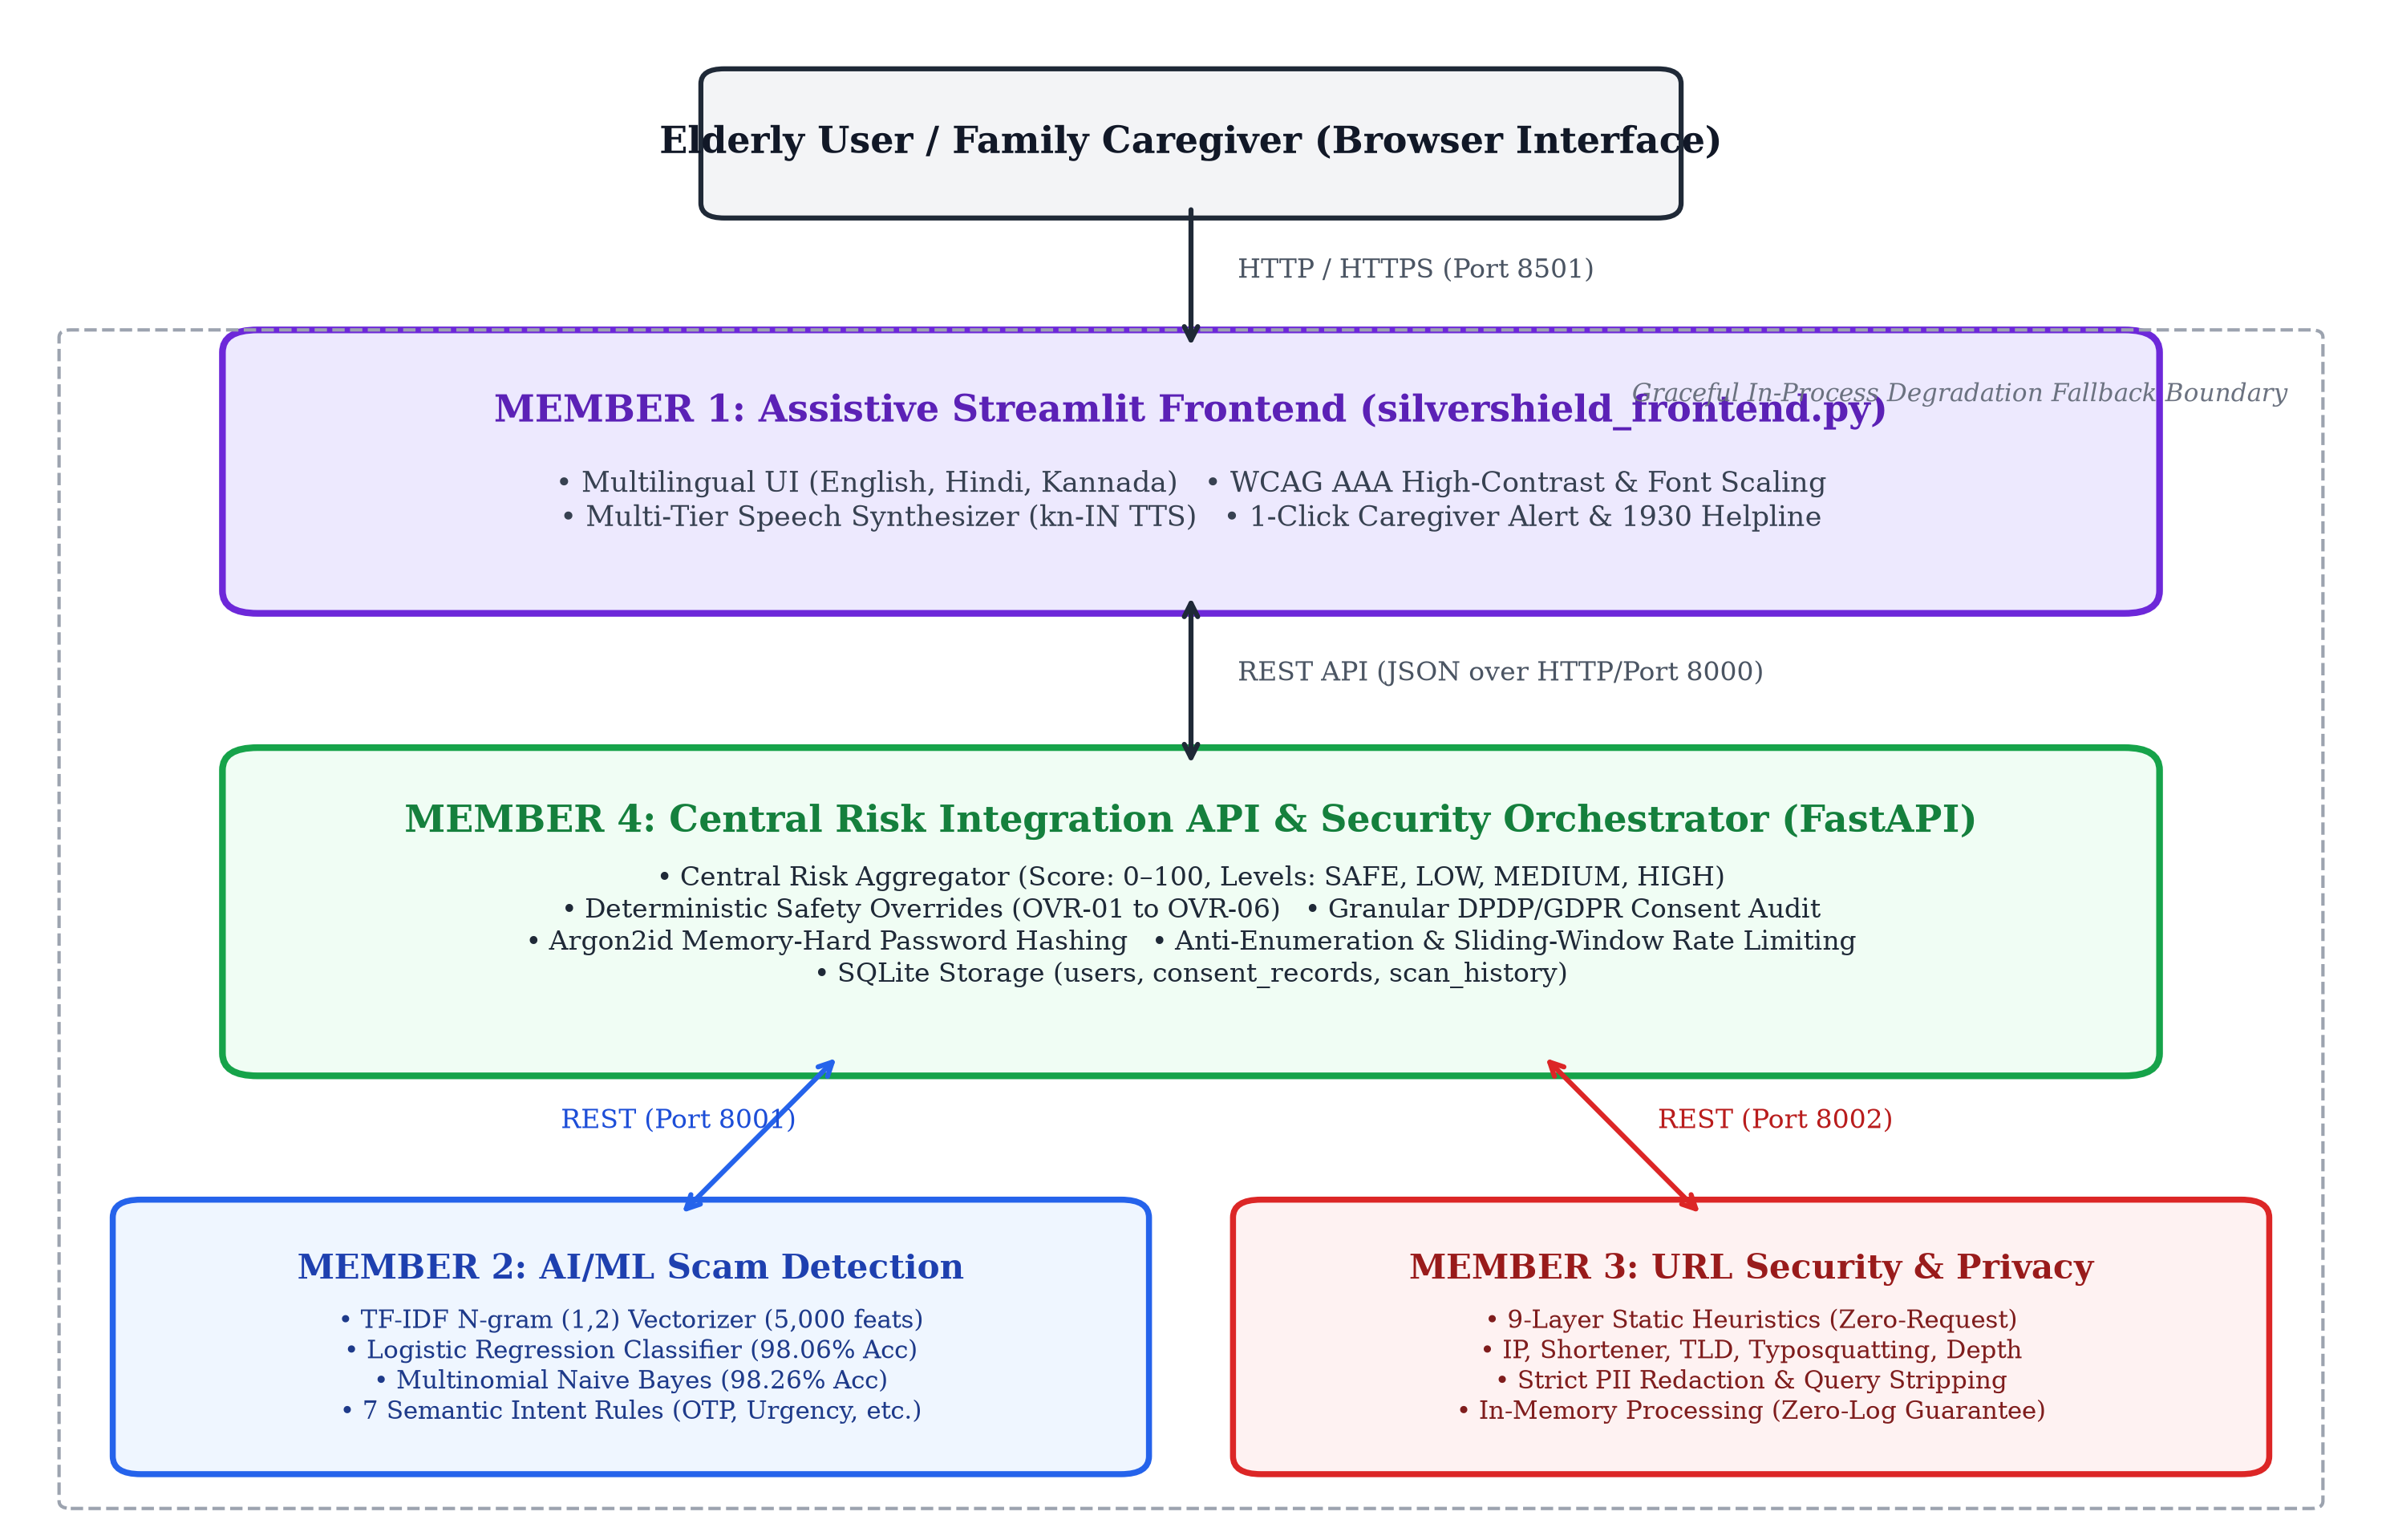
\includegraphics[width=\columnwidth]{images/fig1_system_architecture.png}
\caption{Overall System Architecture of SilverShield AI illustrating the 4-tier microservice topology, port assignments, and graceful in-process degradation fallback boundary.}
\label{fig:arch}
\end{figure}

The platform comprises four discrete functional tiers:
\begin{enumerate}
    \item \textbf{Presentation Tier (Port 8501):} Built with Streamlit, providing reactive UI rendering, font scaling, contrast switching, and browser-native Web Speech narration.
    \item \textbf{Integration and Security Tier (Port 8000):} Developed with FastAPI, hosting the central risk engine, Argon2id authentication, rate limiting, and SQLite storage.
    \item \textbf{AI/ML Scam Detection Tier (Port 8001):} A dedicated FastAPI service running TF-IDF feature extraction, Logistic Regression inference, and intent indicator parsing.
    \item \textbf{URL Security Tier (Port 8002):} A dedicated FastAPI service executing 9-layer static heuristic inspections, query parameter redaction, and PII scrubbing.
\end{enumerate}

\subsection{System Workflow}
The end-to-end execution pipeline of SilverShield AI follows a structured multi-stage trajectory, depicted in Fig.~\ref{fig:workflow}.

\begin{figure}[t]
\centering
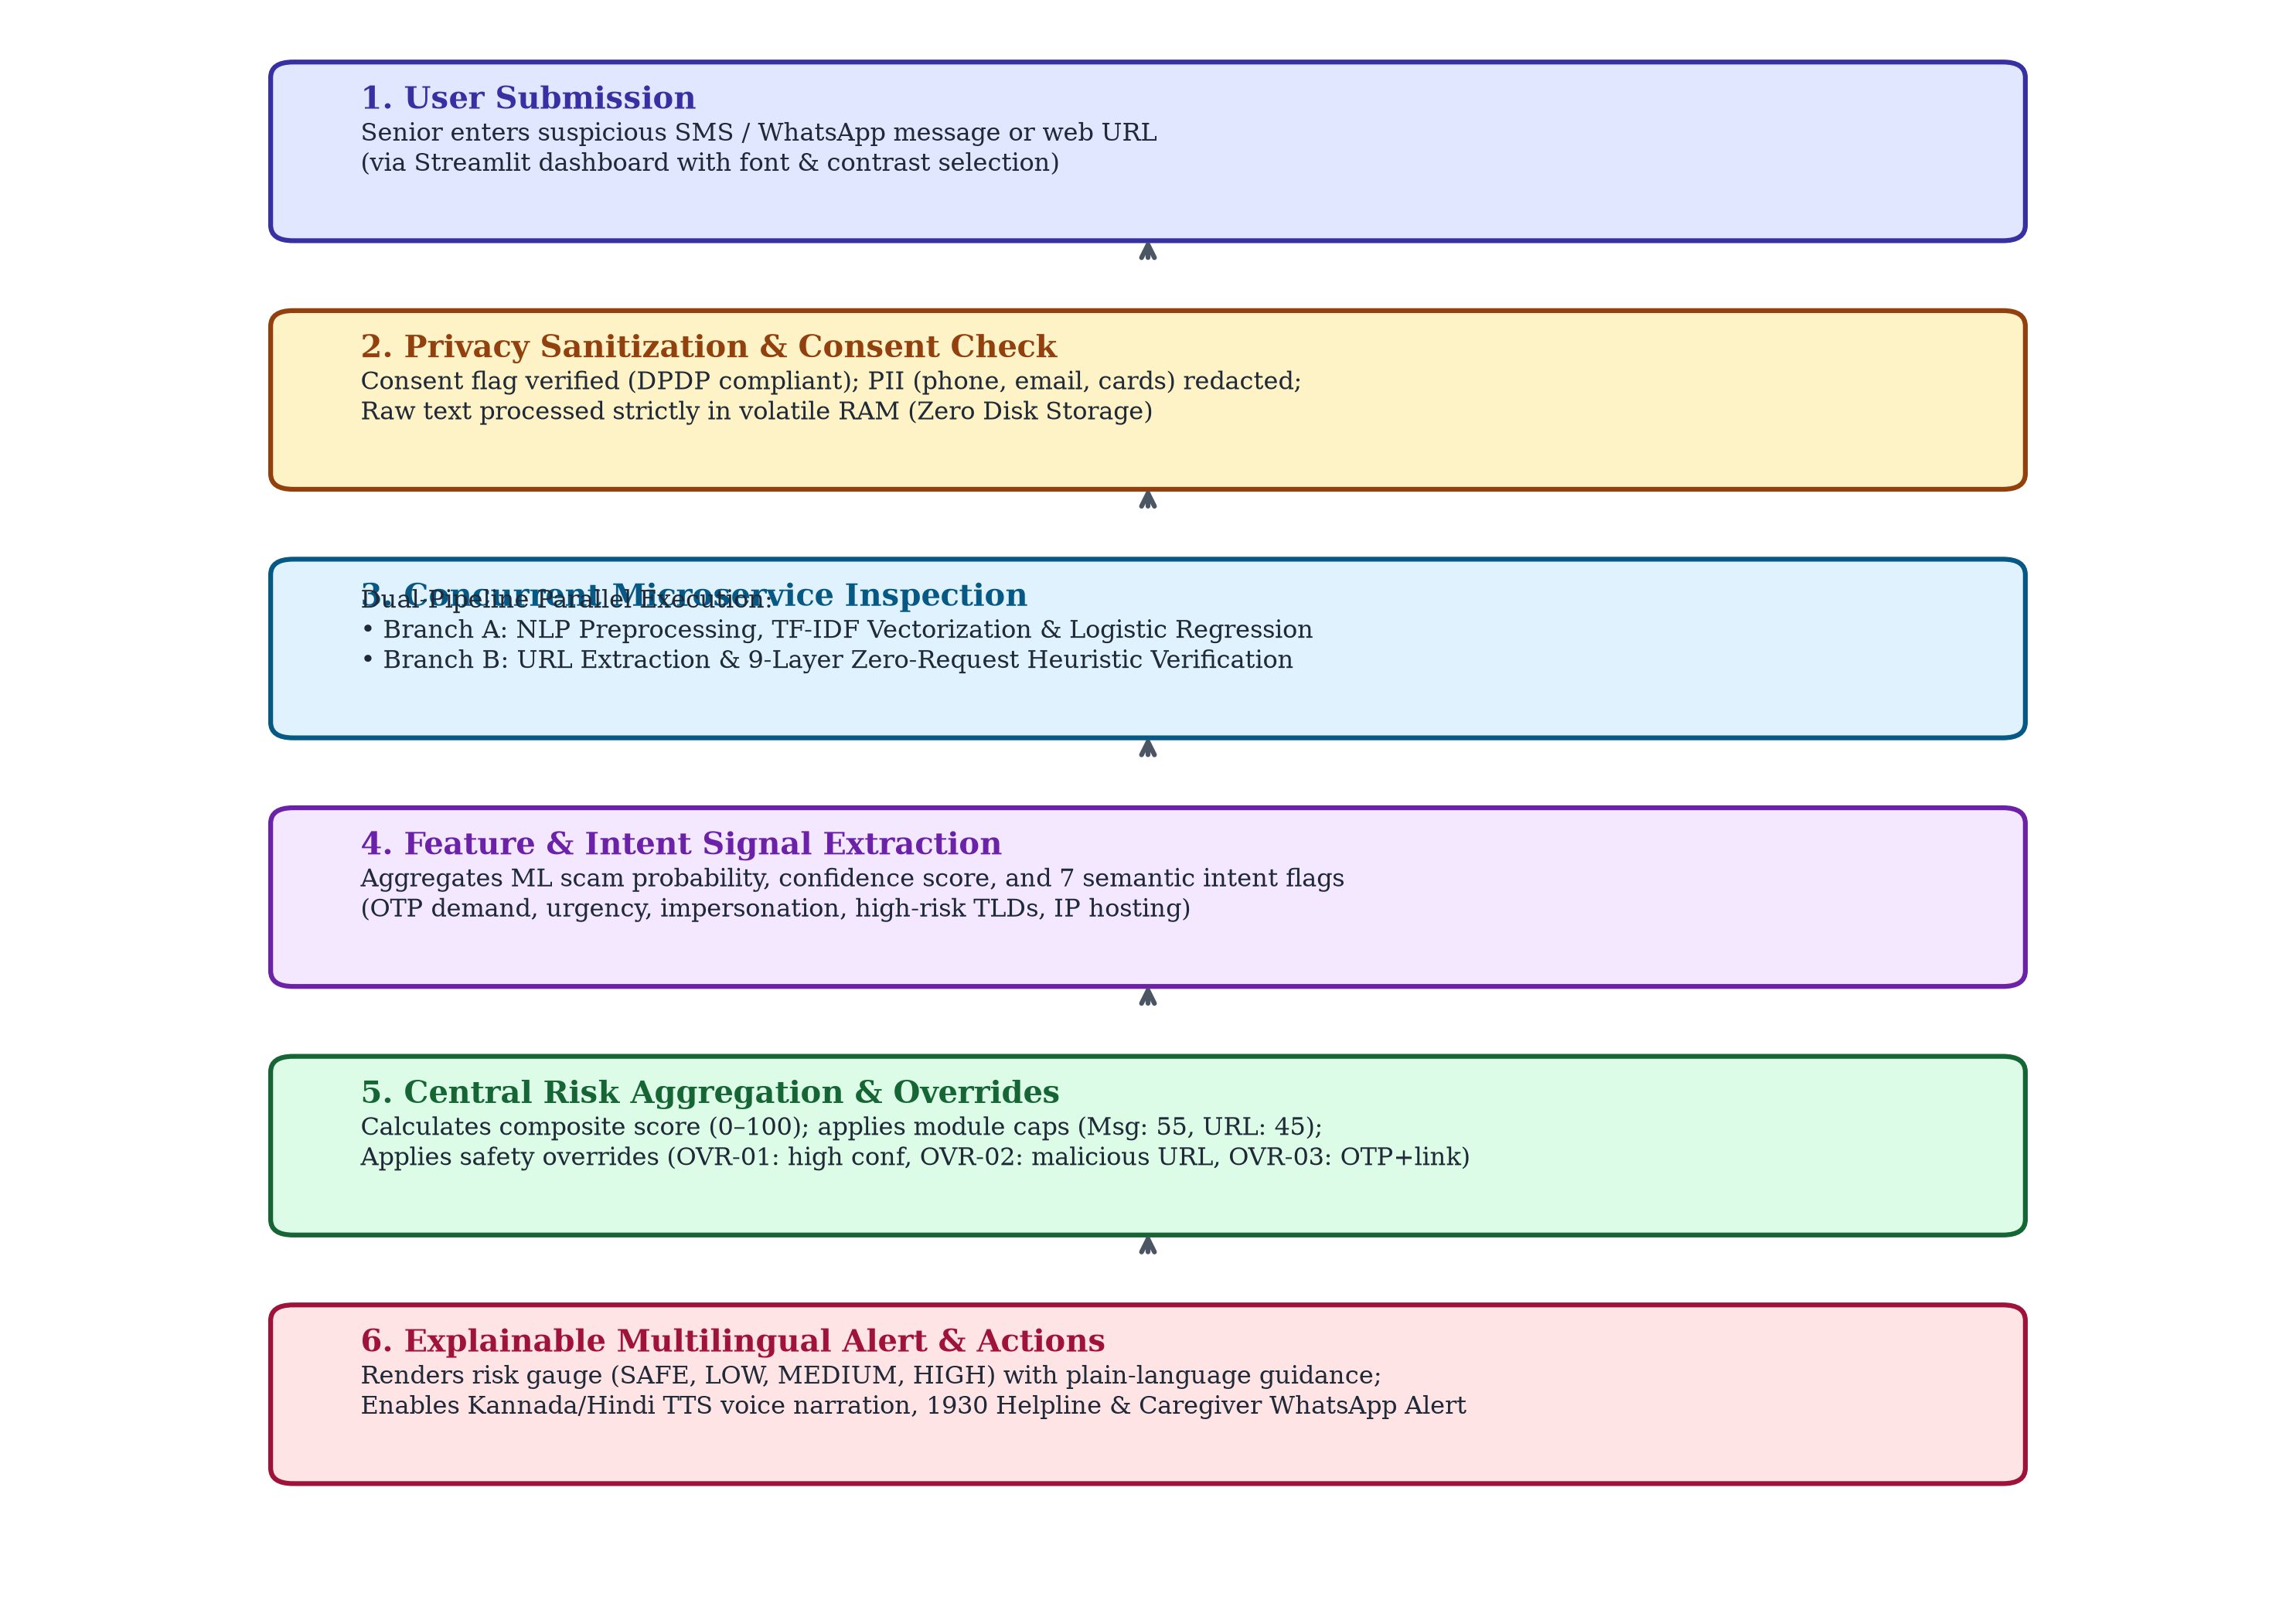
\includegraphics[width=\columnwidth]{images/fig2_system_workflow.png}
\caption{End-to-End System Workflow Diagram depicting user submission, privacy validation, parallel microservice analysis, risk score aggregation, and multilingual assistive output.}
\label{fig:workflow}
\end{figure}

When a senior user submits an SMS or WhatsApp message:
\begin{enumerate}
    \item The frontend verifies that consent is granted and executes client-side whitespace normalization.
    \item The payload is transmitted to the central orchestrator (Port 8000), which checks payload boundaries ($\le 64$\,KB) and strips personal identifiable information (PII).
    \item The orchestrator concurrently dispatches the text to the ML Scam Engine (Port 8001) and any extracted hyperlinks to the URL Security API (Port 8002).
    \item Signals from both microservices are aggregated into a composite risk score governed by source caps and safety overrides.
    \item The final response delivers the categorical risk level, threat indicators, plain-language warnings, actionable steps, and regional voice narration.
\end{enumerate}

\subsection{Frontend Implementation}
The user interface (\texttt{silvershield\_frontend.py}) is crafted using Streamlit with custom CSS and HTML5 embeds (\texttt{frontend/styles.py}). Designed in adherence to human-computer interaction (HCI) standards for seniors:
\begin{itemize}
    \item \textbf{Color Palette:} Deep Purple (\texttt{\#49316F}) provides calming, high-contrast headings; Soft Lavender (\texttt{\#EDE5FA}) defines card backgrounds; and Crimson (\texttt{\#DC2626}) highlights critical dangers.
    \item \textbf{Typography and Touch Targets:} Standard base font of 15\,px with toggleable Large scaling (17\,px). All primary action buttons feature minimum touch heights of 44\,px.
    \item \textbf{WCAG AAA High Contrast:} A dedicated toggle transforms the entire interface into an ultra-high-contrast deep dark palette (\texttt{\#0B0814} background, \texttt{\#FFFFFF} text, \texttt{\#B39DDB} borders) achieving a contrast ratio $>7:1$.
    \item \textbf{Minimal Cognitive Friction:} Navigation is housed within an unobtrusive top-right menu ($\vdots$), removing clutter and confusing technical dials.
\end{itemize}

\subsection{Backend Implementation}
The central integration backend (\texttt{app/main.py}) is implemented using FastAPI and served via Uvicorn. Inter-service HTTP requests are managed through resilient HTTPX/Requests adapters configured with 1.0-second timeout guards and zero retries to prevent blocking worker threads. If a microservice fails to respond within the allocated threshold, the orchestrator triggers \textbf{Graceful In-Process Degradation}:
\begin{itemize}
    \item If the ML Scam Engine (Port 8001) is unreachable, the orchestrator logs state as \texttt{UNAVAILABLE}, flags system status as \texttt{DEGRADED}, and sets a mandatory risk floor of \texttt{MEDIUM}.
    \item If the URL Security API (Port 8002) is offline, URL status reports \texttt{UNKNOWN} while textual scam classification proceeds unhindered.
    \item If the entire central API (Port 8000) is offline, the Streamlit frontend automatically activates its embedded \textbf{Local AI Security Engine}, executing identical Scikit-Learn models and URL heuristics in-process.
\end{itemize}

\subsection{AI/ML Implementation}
The AI/ML scam detection architecture (\texttt{ai\_module/src/}) processes informal mobile texts to distinguish between benign communications and fraudulent lures. The end-to-end training and inference pipeline is illustrated in Fig.~\ref{fig:ml_workflow}.

\begin{figure}[t]
\centering
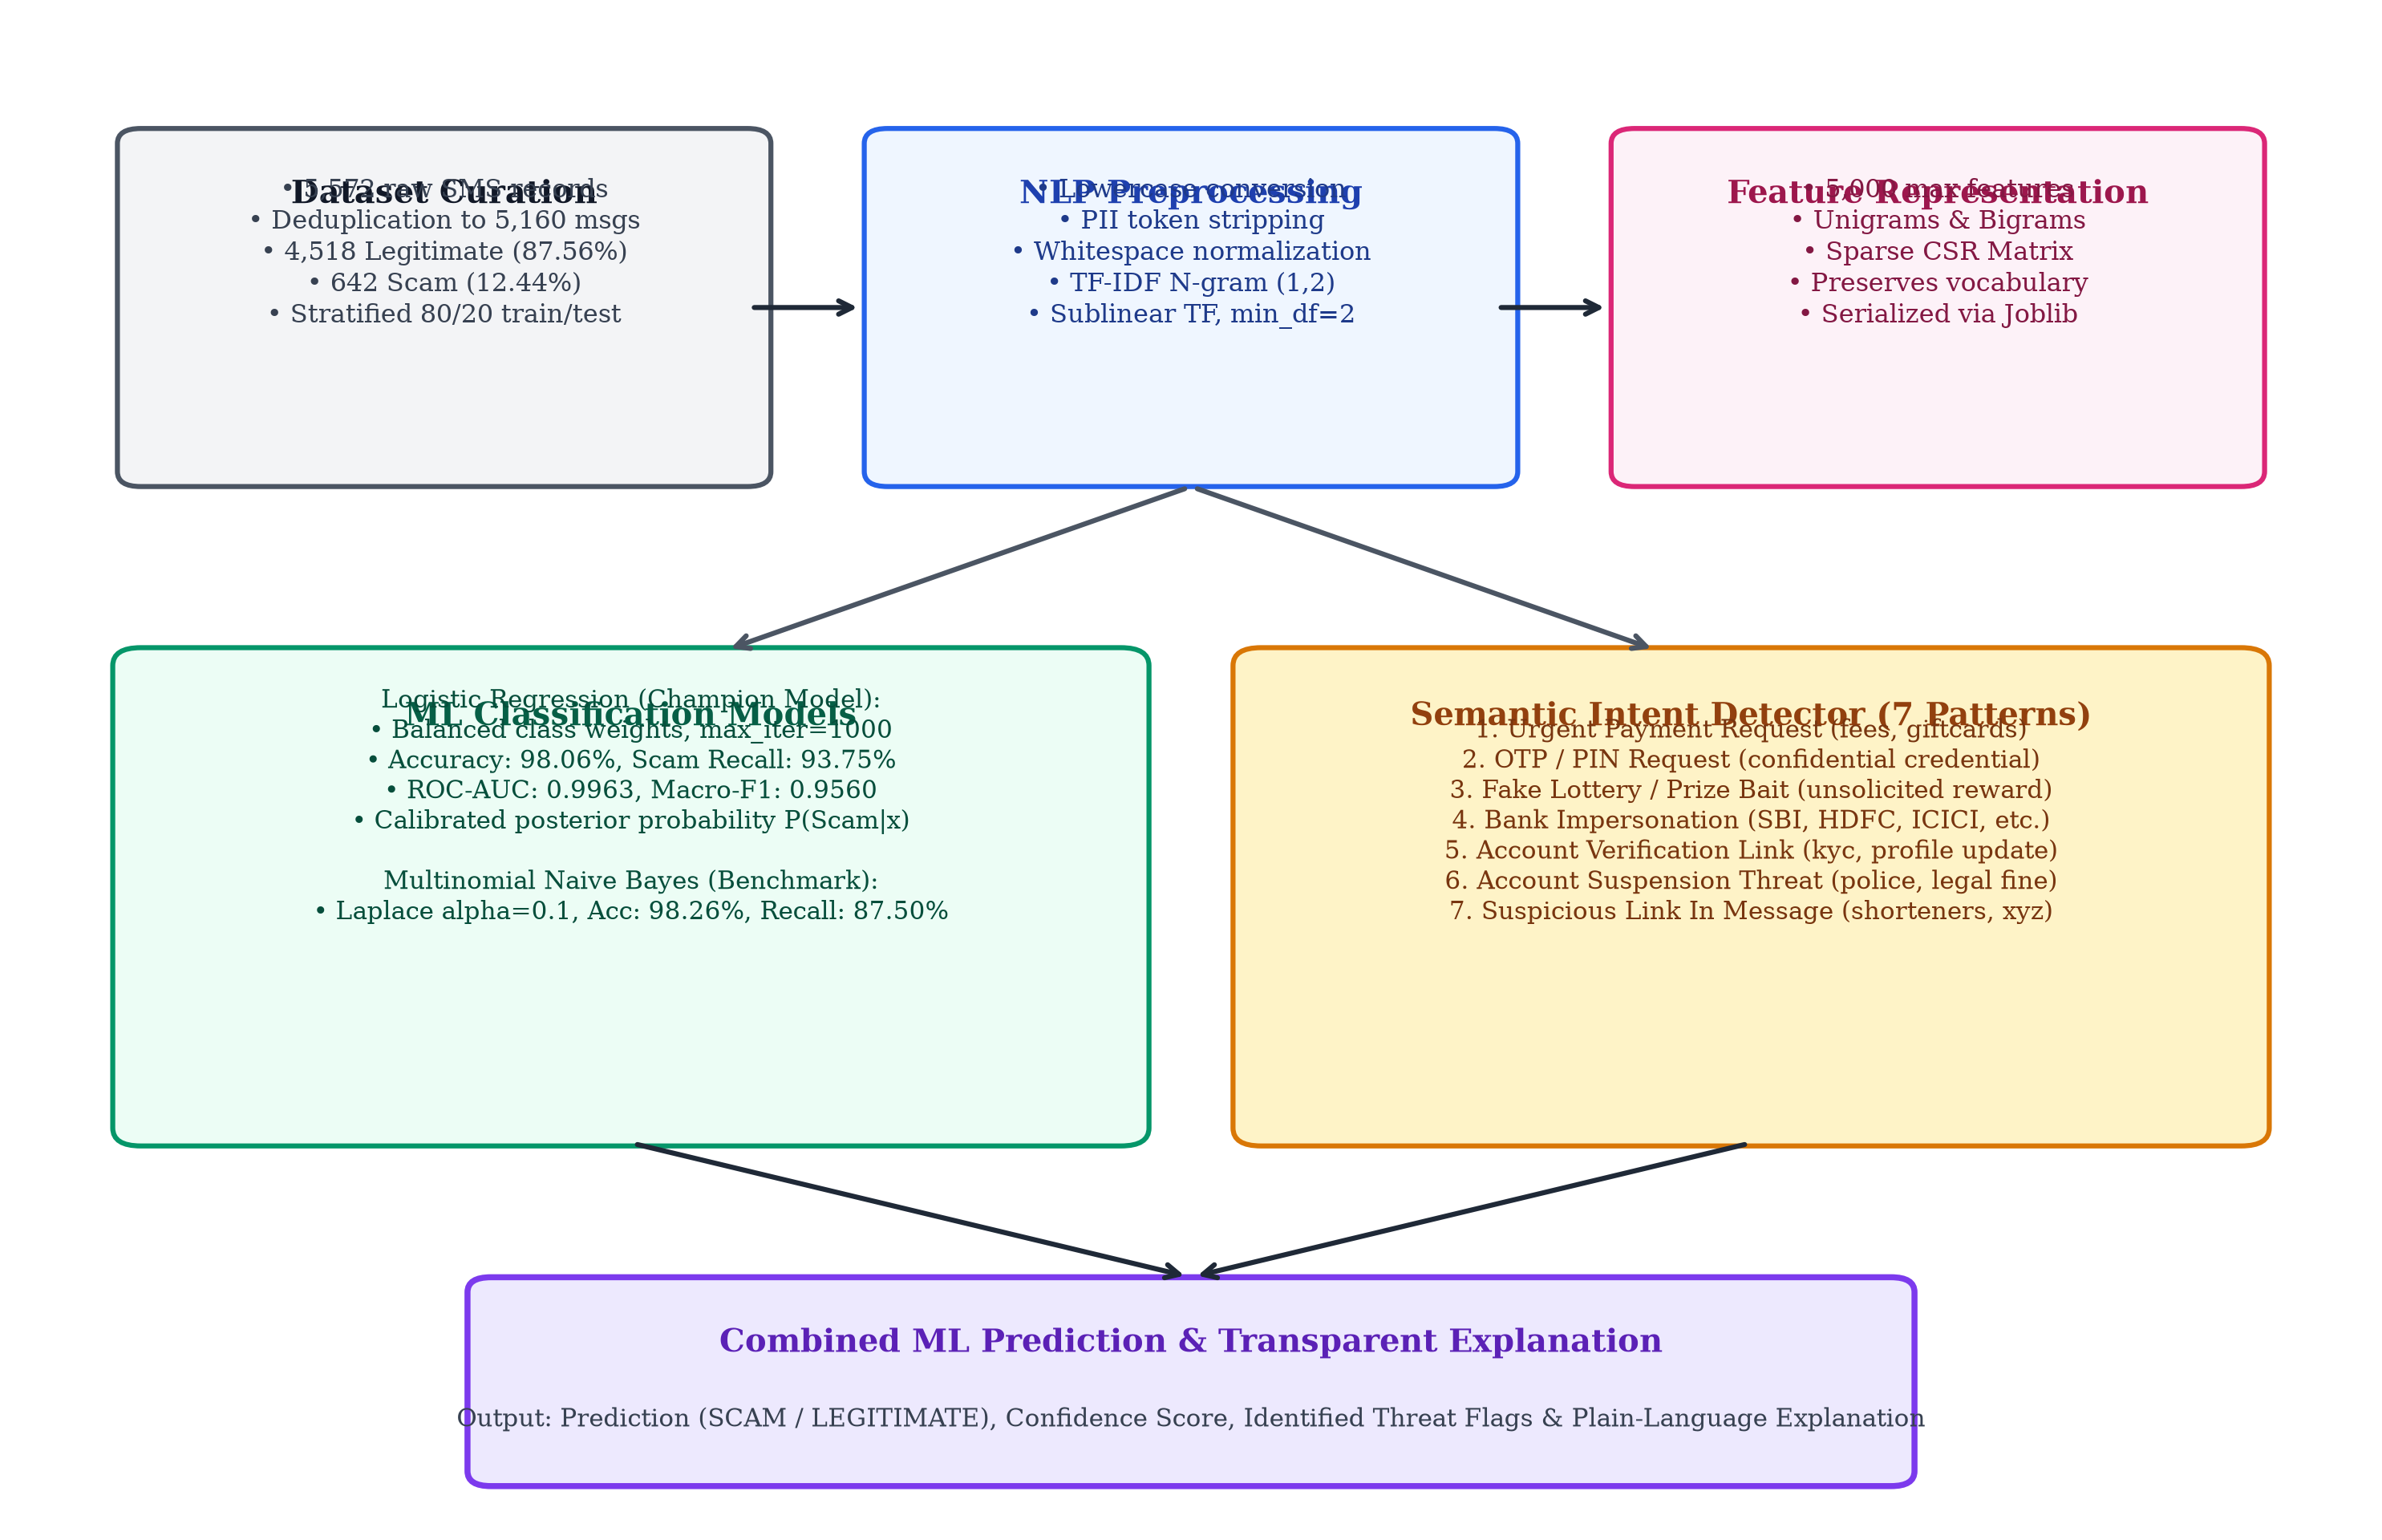
\includegraphics[width=\columnwidth]{images/fig3_ml_workflow.png}
\caption{AI/ML Scam Message Detection Pipeline illustrating dataset curation, TF-IDF vectorization, Logistic Regression classification, and 7-pattern semantic intent extraction.}
\label{fig:ml_workflow}
\end{figure}

\subsection{Dataset Description}
The machine learning subsystem is trained on a curated corpus derived from the benchmark SMS Spam Collection \cite{almeida2011contributions}. The raw dataset comprises 5,572 mobile messages. Rigorous data hygiene and deduplication yielded 5,160 unique records, summarized in Table~\ref{tab:dataset}.

\begin{table}[h]
\caption{Dataset Description and Class Distribution}
\label{tab:dataset}
\centering
\small
\begin{tabular}{lrr}
\toprule
\textbf{Dataset Attribute} & \textbf{Value / Count} & \textbf{Percentage} \\
\midrule
Raw Corpus Records & 5,572 & 100.00\% \\
Deduplicated Unique Messages & 5,160 & 100.00\% \\
Legitimate Class (\textit{Ham}) & 4,518 & 87.56\% \\
Scam / Fraud Class (\textit{Spam}) & 642 & 12.44\% \\
Training Partition (80\%, Stratified) & 4,128 & 80.00\% \\
Testing Partition (20\%, Stratified) & 1,032 & 20.00\% \\
Test Partition: Legitimate & 904 & 87.60\% \\
Test Partition: Scam & 128 & 12.40\% \\
\bottomrule
\end{tabular}
\end{table}

\subsection{Data Preprocessing}
Text normalization (\texttt{ai\_module/src/preprocessing.py}) executes sequentially:
\begin{enumerate}
    \item \textbf{Case Folding:} All string characters are converted to lowercase.
    \item \textbf{PII Stripping:} Phone numbers, email addresses, and credit card patterns are sanitized to prevent memorization of specific phone numbers.
    \item \textbf{Whitespace Normalization:} Redundant tabs, trailing line breaks, and multi-spaces are collapsed.
    \item \textbf{Boundary Guarding:} Messages shorter than 2 characters or exceeding 1,000 characters are rejected.
\end{enumerate}

\subsection{TF-IDF Feature Extraction}
Text representations are constructed using Scikit-Learn's \texttt{TfidfVectorizer}:
\begin{itemize}
    \item \textbf{N-gram Range:} Unigrams and bigrams (\texttt{ngram\_range=(1, 2)}) to capture contextual compound phrases such as ``account blocked'', ``verify kyc'', and ``free cash''.
    \item \textbf{Term Frequency Scaling:} Sublinear TF scaling ($1 + \log(\text{tf})$) to dampen the distorting impact of repeated tokens.
    \item \textbf{Frequency Thresholds:} Minimum document frequency of $\text{min\_df} = 2$ and maximum features capped at 5,000 top informative dimensions.
\end{itemize}

\subsection{Machine Learning Algorithms}
Two supervised learning classifiers were configured, trained, and benchmarked:
\begin{enumerate}
    \item \textbf{Logistic Regression (Champion Model):} Configured with balanced class weights (\texttt{class\_weight='balanced'}) to address the 87.56\% vs 12.44\% class imbalance, \texttt{max\_iter=1000}, and random seed 42. Logistic Regression outputs calibrated posterior probabilities via the standard sigmoid activation:
    \begin{equation}
    P(y = 1 \mid \mathbf{x}) = \frac{1}{1 + e^{-(\mathbf{w}^T \mathbf{x} + b)}}
    \label{eq:lr}
    \end{equation}
    where $\mathbf{x} \in \mathbb{R}^{5000}$ represents the sparse TF-IDF vector, $\mathbf{w}$ denotes the learned weight vector, and $b$ is the scalar bias. A message is classified as \texttt{SCAM} when $P(y = 1 \mid \mathbf{x}) \ge 0.50$. The prediction confidence is defined as:
    \begin{equation}
    \text{Confidence} = \max\bigl(P(y = 1 \mid \mathbf{x}),\, 1 - P(y = 1 \mid \mathbf{x})\bigr)
    \end{equation}
    \item \textbf{Multinomial Naive Bayes (Benchmark):} Configured with Laplace smoothing parameter $\alpha = 0.1$ and learned class priors.
\end{enumerate}

\subsection{Scam Message Detection}
Beyond probabilistic classification, the module incorporates a deterministic intent detector (\texttt{ai\_module/src/warning\_indicators.py}) scanning for 7 semantic deception categories:
\begin{enumerate}
    \item \texttt{urgent\_payment}: Pressures users to transfer funds, settle courier fees, or purchase gift cards.
    \item \texttt{otp\_request}: Demands one-time passwords, PINs, or security passcodes.
    \item \texttt{fake\_prize}: Unsolicited lottery wins, cashback vouchers, or gift rewards.
    \item \texttt{bank\_impersonation}: Claims of representing SBI, HDFC, ICICI, Axis, or central banks.
    \item \texttt{account\_verification}: Urges verification of identity, credentials, or KYC records.
    \item \texttt{account\_suspension}: Threats of account closure, SIM deactivation, or police warrants.
    \item \texttt{suspicious\_link}: Presence of shortened links or deceptive domains within text.
\end{enumerate}

\subsection{Suspicious URL Analysis}
The URL Security Engine (\texttt{url\_analysis/analyzer.py}) inspects web hyperlinks using 9 zero-request static heuristic layers, illustrated in Fig.~\ref{fig:url_workflow}.

\begin{figure}[t]
\centering
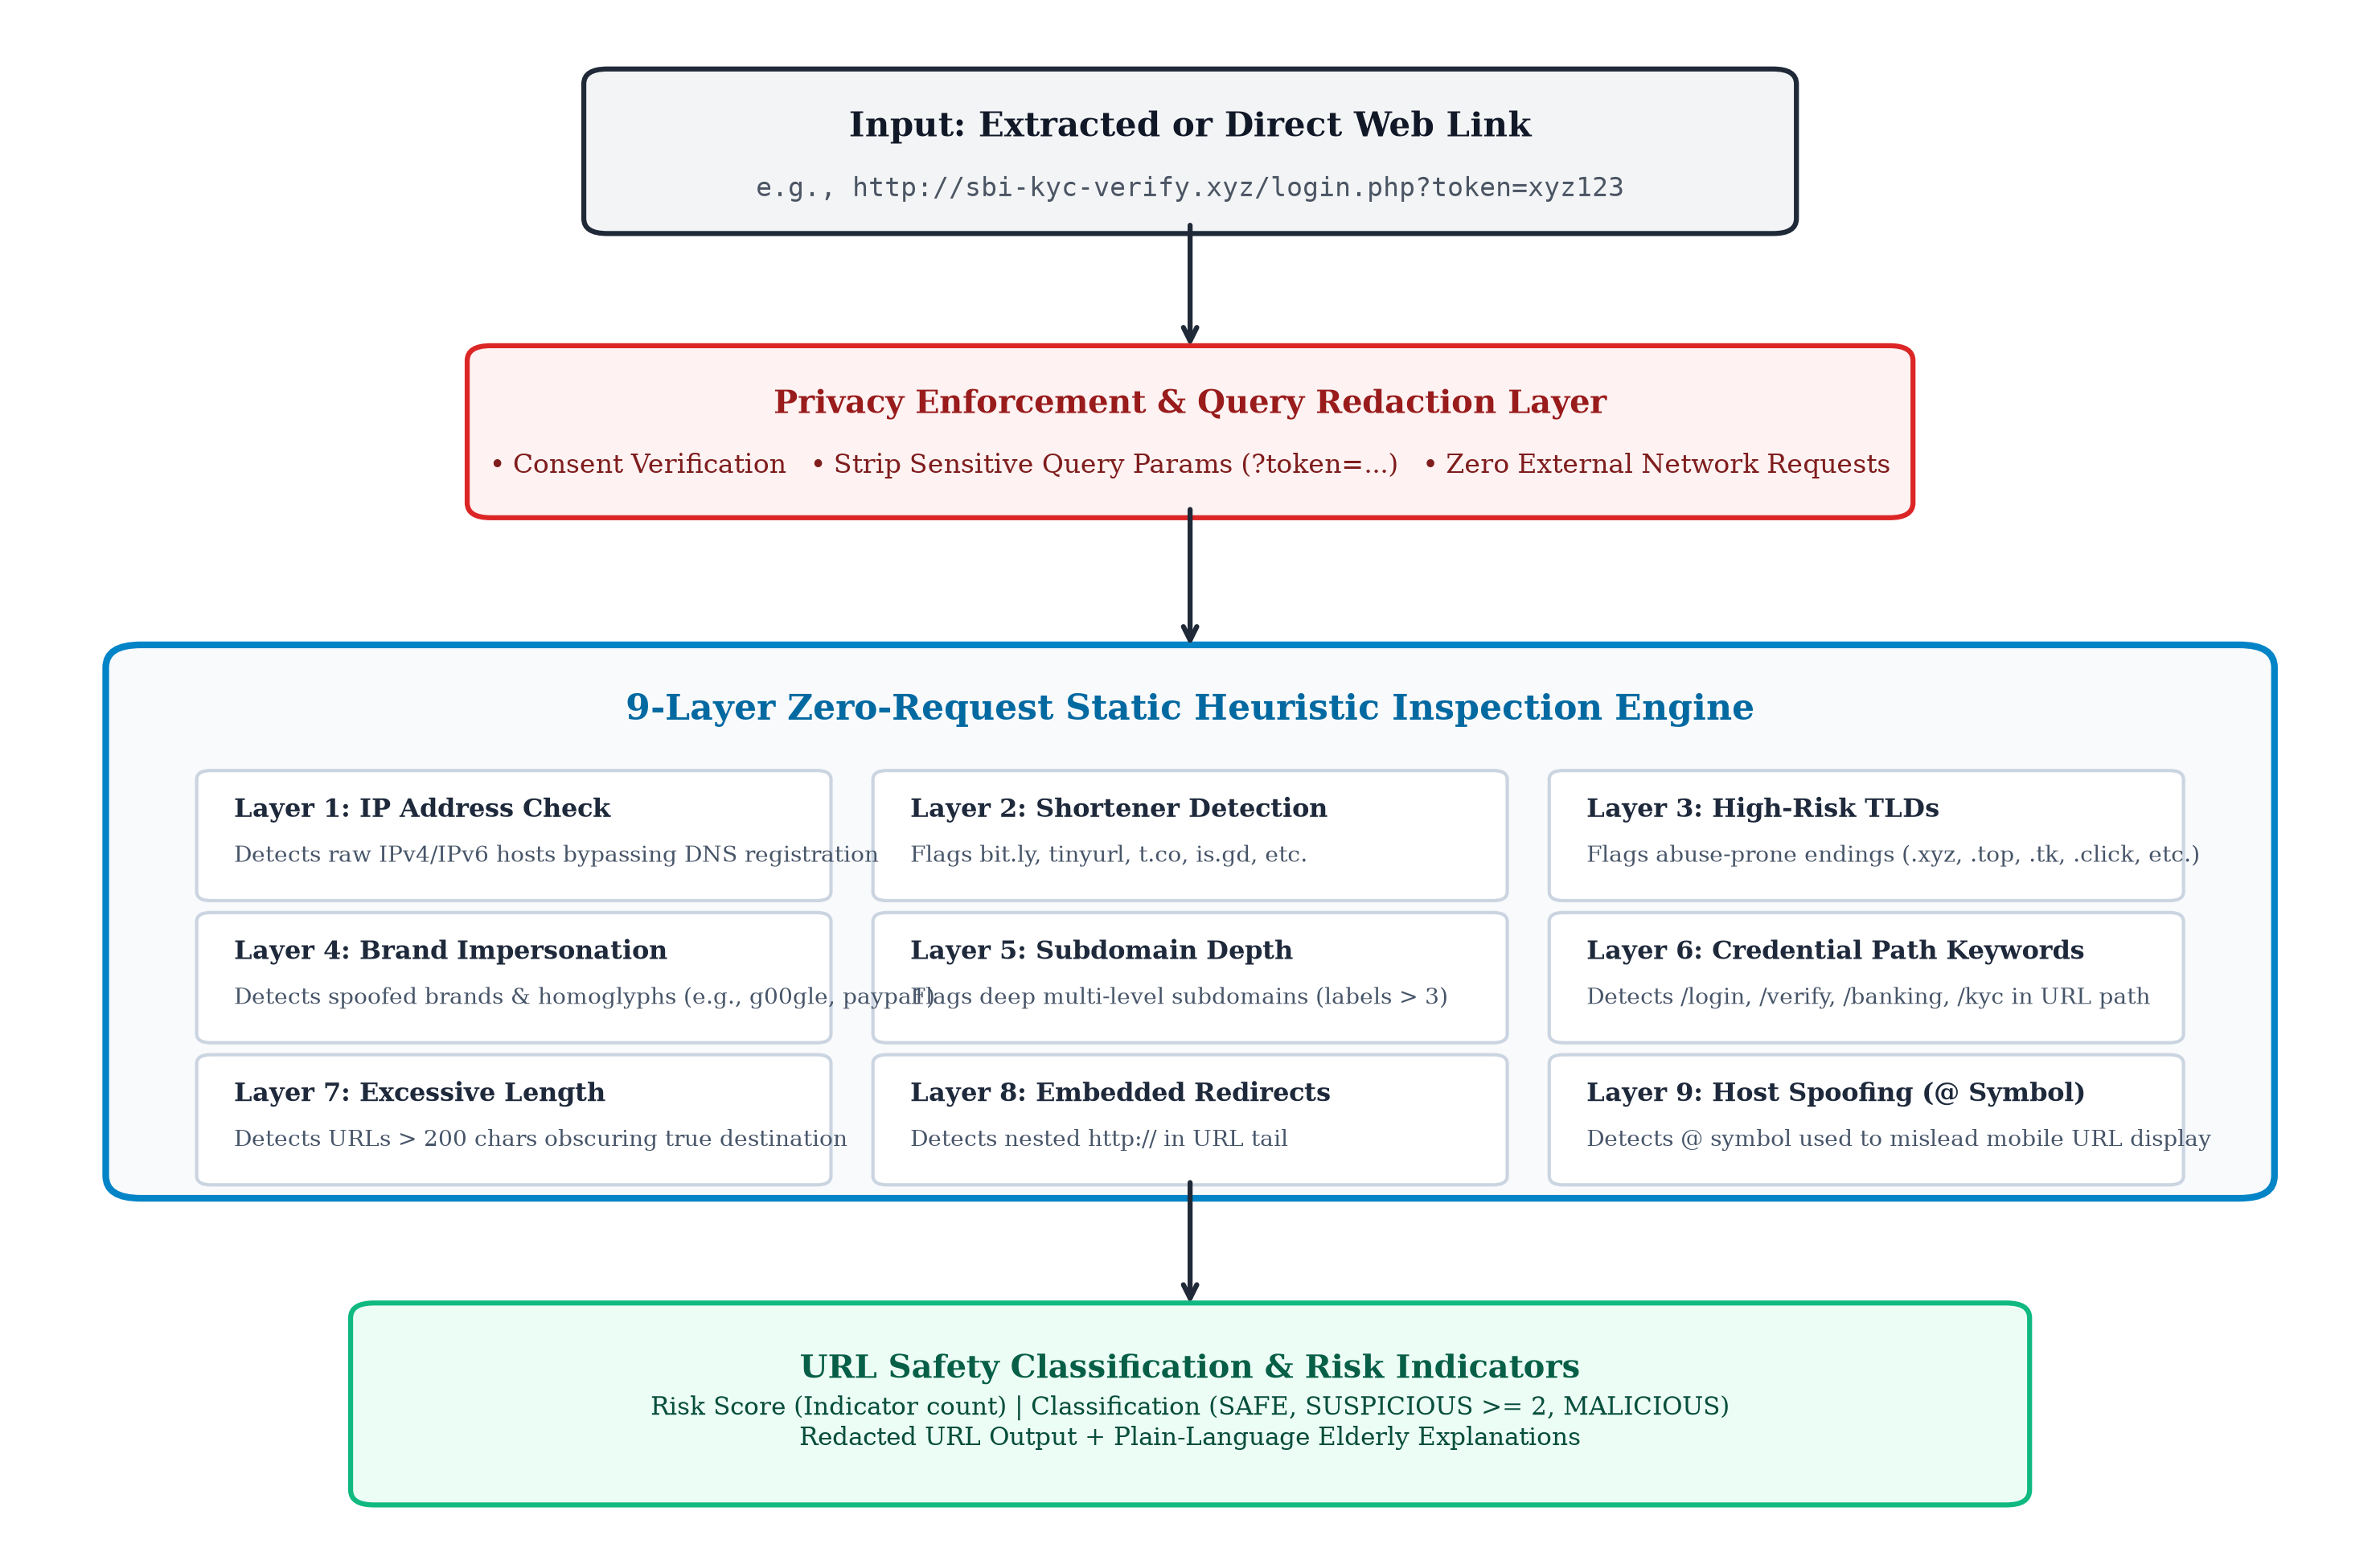
\includegraphics[width=\columnwidth]{images/fig4_url_workflow.png}
\caption{Suspicious URL Analysis Workflow detailing PII redaction, query string stripping, and the 9 zero-request static heuristic inspection layers.}
\label{fig:url_workflow}
\end{figure}

The 9 inspection layers operate strictly in memory:
\begin{enumerate}
    \item \textbf{IP Address Host:} Regex matches direct IPv4/IPv6 hosts (e.g., \texttt{http://192.168.0.1/login}) used to bypass DNS domain reputation filters.
    \item \textbf{URL Shorteners:} Checks against 16 known shortening hosts (\texttt{bit.ly}, \texttt{tinyurl.com}, \texttt{t.co}, \texttt{is.gd}, etc.).
    \item \textbf{High-Risk TLDs:} Evaluates extensions commonly abused in smishing (\texttt{.xyz}, \texttt{.top}, \texttt{.club}, \texttt{.work}, \texttt{.click}, \texttt{.zip}).
    \item \textbf{Brand Impersonation / Homoglyphs:} Strips digits and identifies deceptive brand variations targeting 21 major entities (e.g., \texttt{paypal}, \texttt{amazon}, \texttt{sbi}, \texttt{chase}).
    \item \textbf{Subdomain Depth:} Flags nesting depth exceeding 3 labels (e.g., \texttt{login.verify.bank.secure.com}).
    \item \textbf{Suspicious Path Keywords:} Scans URL path strings for credential-harvesting tokens (\texttt{login}, \texttt{signin}, \texttt{verify}, \texttt{banking}, \texttt{kyc}).
    \item \textbf{Excessive Length:} Flags URLs exceeding 200 characters designed to push domain names off mobile screens.
    \item \textbf{Embedded Redirects:} Identifies nested \texttt{http} protocol markers in the query tail.
    \item \textbf{Host Spoofing (@ Symbol):} Flags \texttt{@} characters in authority components used to disguise destination hosts.
\end{enumerate}
To preserve user privacy, query strings and session fragments are stripped prior to reporting:
\begin{equation}
\text{\texttt{http://scam.xyz/pay?user=senior\&token=9928}} \;\to\; \text{\texttt{http://scam.xyz/pay}}
\end{equation}

\subsection{Risk Assessment Engine}
Implemented in \texttt{app/core/risk\_engine.py}, the central risk engine translates signals into a unified threat score ($0$--$100$) and four categorical risk levels, depicted in Fig.~\ref{fig:risk_workflow}.

\begin{figure}[t]
\centering
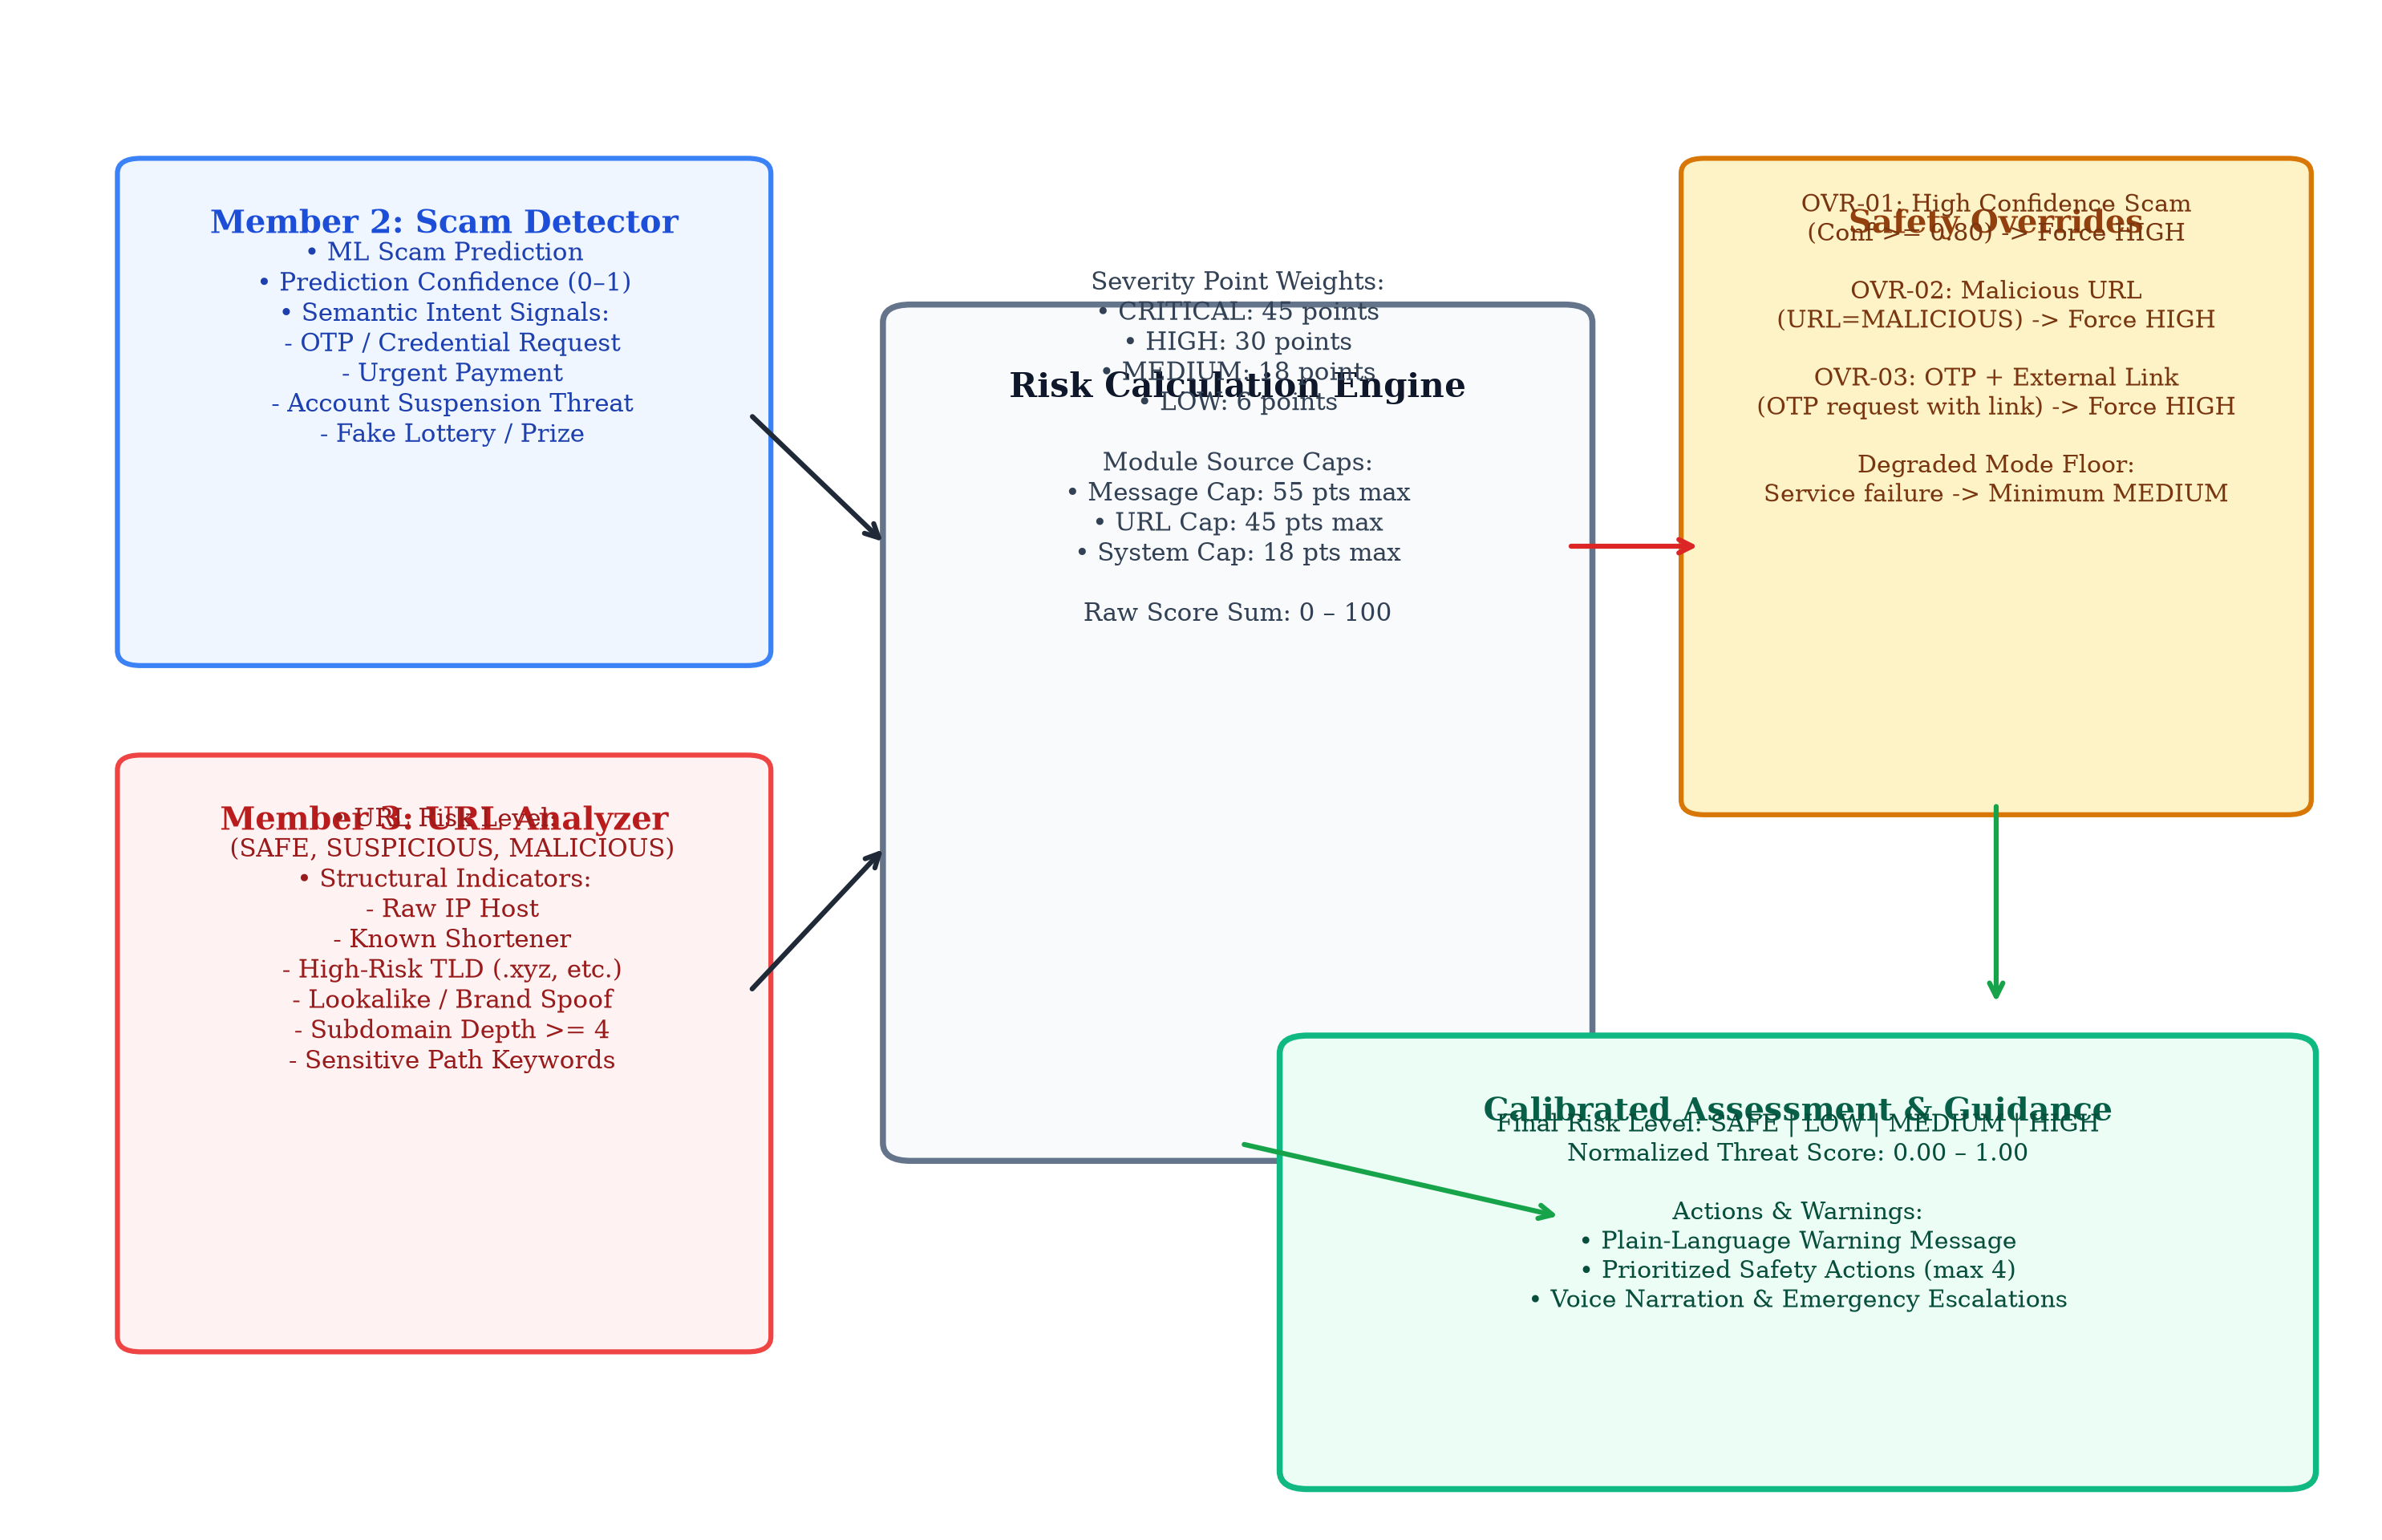
\includegraphics[width=\columnwidth]{images/fig5_risk_assessment_workflow.png}
\caption{Central Risk Assessment Workflow showing point allocation, module source caps, deterministic safety overrides, and final action mapping.}
\label{fig:risk_workflow}
\end{figure}

Points are assigned according to threat severity:
\begin{itemize}
    \item \texttt{CRITICAL} Indicators: 45 points each.
    \item \texttt{HIGH} Indicators: 30 points each.
    \item \texttt{MEDIUM} Indicators: 18 points each.
    \item \texttt{LOW} Indicators: 6 points each.
\end{itemize}
To prevent a single anomalous indicator from distorting results, contributions are capped per module source:
\begin{equation}
\text{Total Score} = \min(55, S_{\text{msg}}) + \min(45, S_{\text{url}}) + \min(18, S_{\text{sys}})
\end{equation}
Baseline categorical thresholds:
\begin{itemize}
    \item $\text{Score} < 24 \implies \texttt{LOW}$
    \item $24 \le \text{Score} < 55 \implies \texttt{MEDIUM}$
    \item $\text{Score} \ge 55 \implies \texttt{HIGH}$
\end{itemize}

\subsubsection{Deterministic Safety Overrides}
To guarantee senior protection, critical threat patterns trigger non-negotiable safety overrides:
\begin{itemize}
    \item \textbf{OVR-01 (High Confidence Scam):} If ML prediction is \texttt{SCAM} with confidence $\ge 0.80$, overall risk escalates immediately to \texttt{HIGH}.
    \item \textbf{OVR-02 (Malicious URL):} If URL risk is \texttt{MALICIOUS}, overall risk escalates immediately to \texttt{HIGH}.
    \item \textbf{OVR-03 (OTP Request with Link):} Co-occurrence of an OTP demand and an external URL immediately forces risk to \texttt{HIGH}.
    \item \textbf{OVR-04 (Degraded Mode Floor):} If any subsystem fails, minimum risk is locked at \texttt{MEDIUM}.
\end{itemize}

\subsection{Explainable Warning System}
Rather than displaying technical probabilities, SilverShield AI maps risk categories directly to concrete behavioral instructions (\texttt{config/risk\_config.json}). A maximum of four prioritized actions are presented:
\begin{itemize}
    \item \texttt{NEVER\_SHARE\_OTP}: ``Never share an OTP, PIN or password. No bank, police officer or company will ever ask for it.''
    \item \texttt{DO\_NOT\_TRANSFER\_MONEY}: ``Do not transfer money to anyone you have not confirmed in person.''
    \item \texttt{DO\_NOT\_CLICK\_LINK}: ``Do not click the link. Open the organisation's own official app or type its address yourself.''
    \item \texttt{REPORT\_MESSAGE}: ``Report the message and block the sender, then delete it.''
\end{itemize}

\subsection{Privacy and Security Mechanisms}
Security is implemented across all tiers (\texttt{security/}):
\begin{enumerate}
    \item \textbf{Argon2id Password Hashing:} Complies with OWASP Gold Standards: $\text{time\_cost} = 2$, $\text{memory\_cost} = 65{,}536$\,KiB (64\,MiB RAM), $\text{parallelism} = 1$, and 16-byte random salts.
    \item \textbf{Anti-Enumeration Timing Equalizer:} \texttt{resist\_timing\_enumeration()} executes a dummy Argon2id hash cycle whenever an email is not found, eliminating timing side-channels.
    \item \textbf{Sliding-Window Rate Limiting:} Limits registration to 10 requests/min and login to 15 requests/min per IP.
    \item \textbf{JWT Session Protection:} Stateless tokens signed with HMAC-SHA256 (HS256) expiring in 120 minutes, backed by a server-side revocation blacklist.
    \item \textbf{Zero-Raw-Message Rule:} User messages are processed strictly in volatile RAM. No unencrypted text or private SMS is ever committed to disk or database tables.
\end{enumerate}

\subsection{Database Implementation}
Managed through SQLite3 (\texttt{data/silvershield.db}), the schema enforces foreign keys and cascade deletions across three tables:
\begin{itemize}
    \item \texttt{users}: Stores unique user ID, normalized email, Argon2id password hash, role (\texttt{senior} or \texttt{caregiver}), helper contact details, and timestamps.
    \item \texttt{consent\_records}: Stores unbundled consent preferences, policy version, and timestamped audit logs.
    \item \texttt{scan\_history}: Stores non-PII risk ratings, numerical risk scores, and threat indicator lists.
\end{itemize}

\subsection{Accessibility and Multilingual Support}
SilverShield AI provides comprehensive localization across **English**, **Hindi (हिन्दी)**, and **Kannada (ಕನ್ನಡ)** (\texttt{frontend/locales.py}).
The audio narration engine (\texttt{frontend/components.py}) implements a resilient multi-tier strategy:
\begin{enumerate}
    \item Dynamically queries browser speech synthesis voices for regional tags (\texttt{kn-IN}, \texttt{hi-IN}, \texttt{en-IN}).
    \item If no regional voice object is installed in the local OS, sets \texttt{utter.lang = 'kn-IN'}, directing Chromium/Edge engines to synthesize native neural cloud speech.
    \item If local speech fails, automatically falls back to an online text-to-speech audio stream with anonymous headers.
    \item Crucially, Kannada text is never fed to an English voice engine, preventing unintelligible audio output.
\end{enumerate}

\subsection{Technologies Used}
The complete software technology stack is detailed in Table~\ref{tab:tech_stack}.

\begin{table}[h]
\caption{Technologies Used in SilverShield AI}
\label{tab:tech_stack}
\centering
\small
\begin{tabular}{llr}
\toprule
\textbf{Component Tier} & \textbf{Technology / Library} & \textbf{Version} \\
\midrule
Execution Runtime & Python & 3.12+ \\
Frontend Framework & Streamlit & 1.30.0+ \\
REST API Framework & FastAPI & 0.110.0+ \\
ASGI Web Server & Uvicorn & 0.27.0+ \\
Schema Validation & Pydantic v2 & 2.6.0+ \\
Machine Learning & Scikit-Learn & 1.4.0+ \\
Model Persistence & Joblib & 1.3.0+ \\
Data Science & Pandas \& NumPy & 2.0+ / 1.24+ \\
Password Hashing & Argon2-cffi (Argon2id) & 23.1.0+ \\
Session Security & PyJWT (HS256) & 2.9.0+ \\
Database Engine & SQLite3 & Native \\
Automated Testing & Pytest & 8.0.0+ \\
Speech Synthesis & Web Speech API & HTML5 Native \\
\bottomrule
\end{tabular}
\end{table}

\section{Results and Discussion}

\subsection{Machine Learning Model Evaluation}
The machine learning classifiers were evaluated on the held-out test partition of 1,032 samples (904 legitimate, 128 scam) using stratified 5-fold cross-validation. Table~\ref{tab:ml_config} specifies the hyperparameter configurations, and Table~\ref{tab:model_perf} summarizes the comparative performance metrics.

\begin{table}[h]
\caption{Machine Learning Model Hyperparameter Configurations}
\label{tab:ml_config}
\centering
\small
\begin{tabular}{ll}
\toprule
\textbf{Parameter} & \textbf{Configured Value} \\
\midrule
TF-IDF N-gram Range & $(1, 2)$ (Unigrams + Bigrams) \\
TF-IDF Sublinear TF & True ($1 + \log(\text{tf})$) \\
TF-IDF Feature Dimension & 5,000 max features \\
TF-IDF Document Frequency & $\text{min\_df} = 2$ \\
Train / Test Split & 80\% Train (4,128), 20\% Test (1,032) \\
Logistic Regression Solver & L-BFGS, $\text{max\_iter} = 1000$ \\
Logistic Regression Weights & Balanced (\texttt{class\_weight='balanced'}) \\
Multinomial Naive Bayes & Laplace smoothing $\alpha = 0.1$ \\
\bottomrule
\end{tabular}
\end{table}

\begin{table}[h]
\caption{Comparative Machine Learning Performance on Test Partition}
\label{tab:model_perf}
\centering
\small
\begin{tabular}{lrr}
\toprule
\textbf{Performance Metric} & \textbf{Logistic Regression} & \textbf{Multinomial NB} \\
\midrule
\textbf{Overall Accuracy} & 98.06\% & 98.26\% \\
\textbf{Scam Precision} & 90.91\% & 98.25\% \\
\textbf{Scam Recall} & \textbf{93.75\%} & 87.50\% \\
\textbf{Scam F1-Score} & 92.31\% & 92.56\% \\
\textbf{Macro-Averaged F1} & 95.60\% & 95.79\% \\
\textbf{ROC-AUC Score} & \textbf{0.9963} & 0.9892 \\
True Positives (Scams Caught) & \textbf{120} & 112 \\
False Negatives (Scams Missed) & \textbf{8} & 16 \\
\textbf{False Negative Rate (FNR)} & \textbf{6.25\%} & 12.50\% \\
True Negatives (Legitimate) & 892 & 902 \\
False Positives (False Alarms) & 12 & 2 \\
False Positive Rate (FPR) & 1.33\% & 0.22\% \\
5-Fold CV Mean Accuracy & 98.33\% & 98.74\% \\
5-Fold CV Mean Macro-F1 & 96.14\% & 97.02\% \\
\bottomrule
\end{tabular}
\end{table}

\subsection{Discussion of Model Selection}
While Multinomial Naive Bayes achieved a fractionally higher raw accuracy (98.26\% vs 98.06\%) and scam precision (98.25\% vs 90.91\%), \textbf{Logistic Regression was explicitly selected as the Champion Model} for SilverShield AI due to the following critical cybersecurity reasons:
\begin{enumerate}
    \item \textbf{Halving the False Negative Rate:} In defensive cybersecurity for vulnerable seniors, a False Negative (failing to detect an actual scam) can lead to catastrophic financial ruin. Multinomial Naive Bayes missed 16 scams ($\text{FNR} = 12.50\%$), whereas Logistic Regression missed only 8 scams ($\text{FNR} = 6.25\%$). Logistic Regression caught 8 additional fraud attempts.
    \item \textbf{Superior ROC-AUC Discriminative Power:} Logistic Regression achieved an exceptional ROC-AUC score of **0.9963** compared to 0.9892 for Naive Bayes, demonstrating near-perfect class separation across diverse decision thresholds.
    \item \textbf{Probabilistic Calibration and Explainability:} Logistic Regression produces well-calibrated posterior probabilities and interpretable linear feature coefficients, allowing individual n-grams to be explained transparently to senior citizens.
\end{enumerate}

Fig.~\ref{fig:charts} illustrates the empirical evaluation charts generated during model benchmarking.

\begin{figure}[t]
\centering
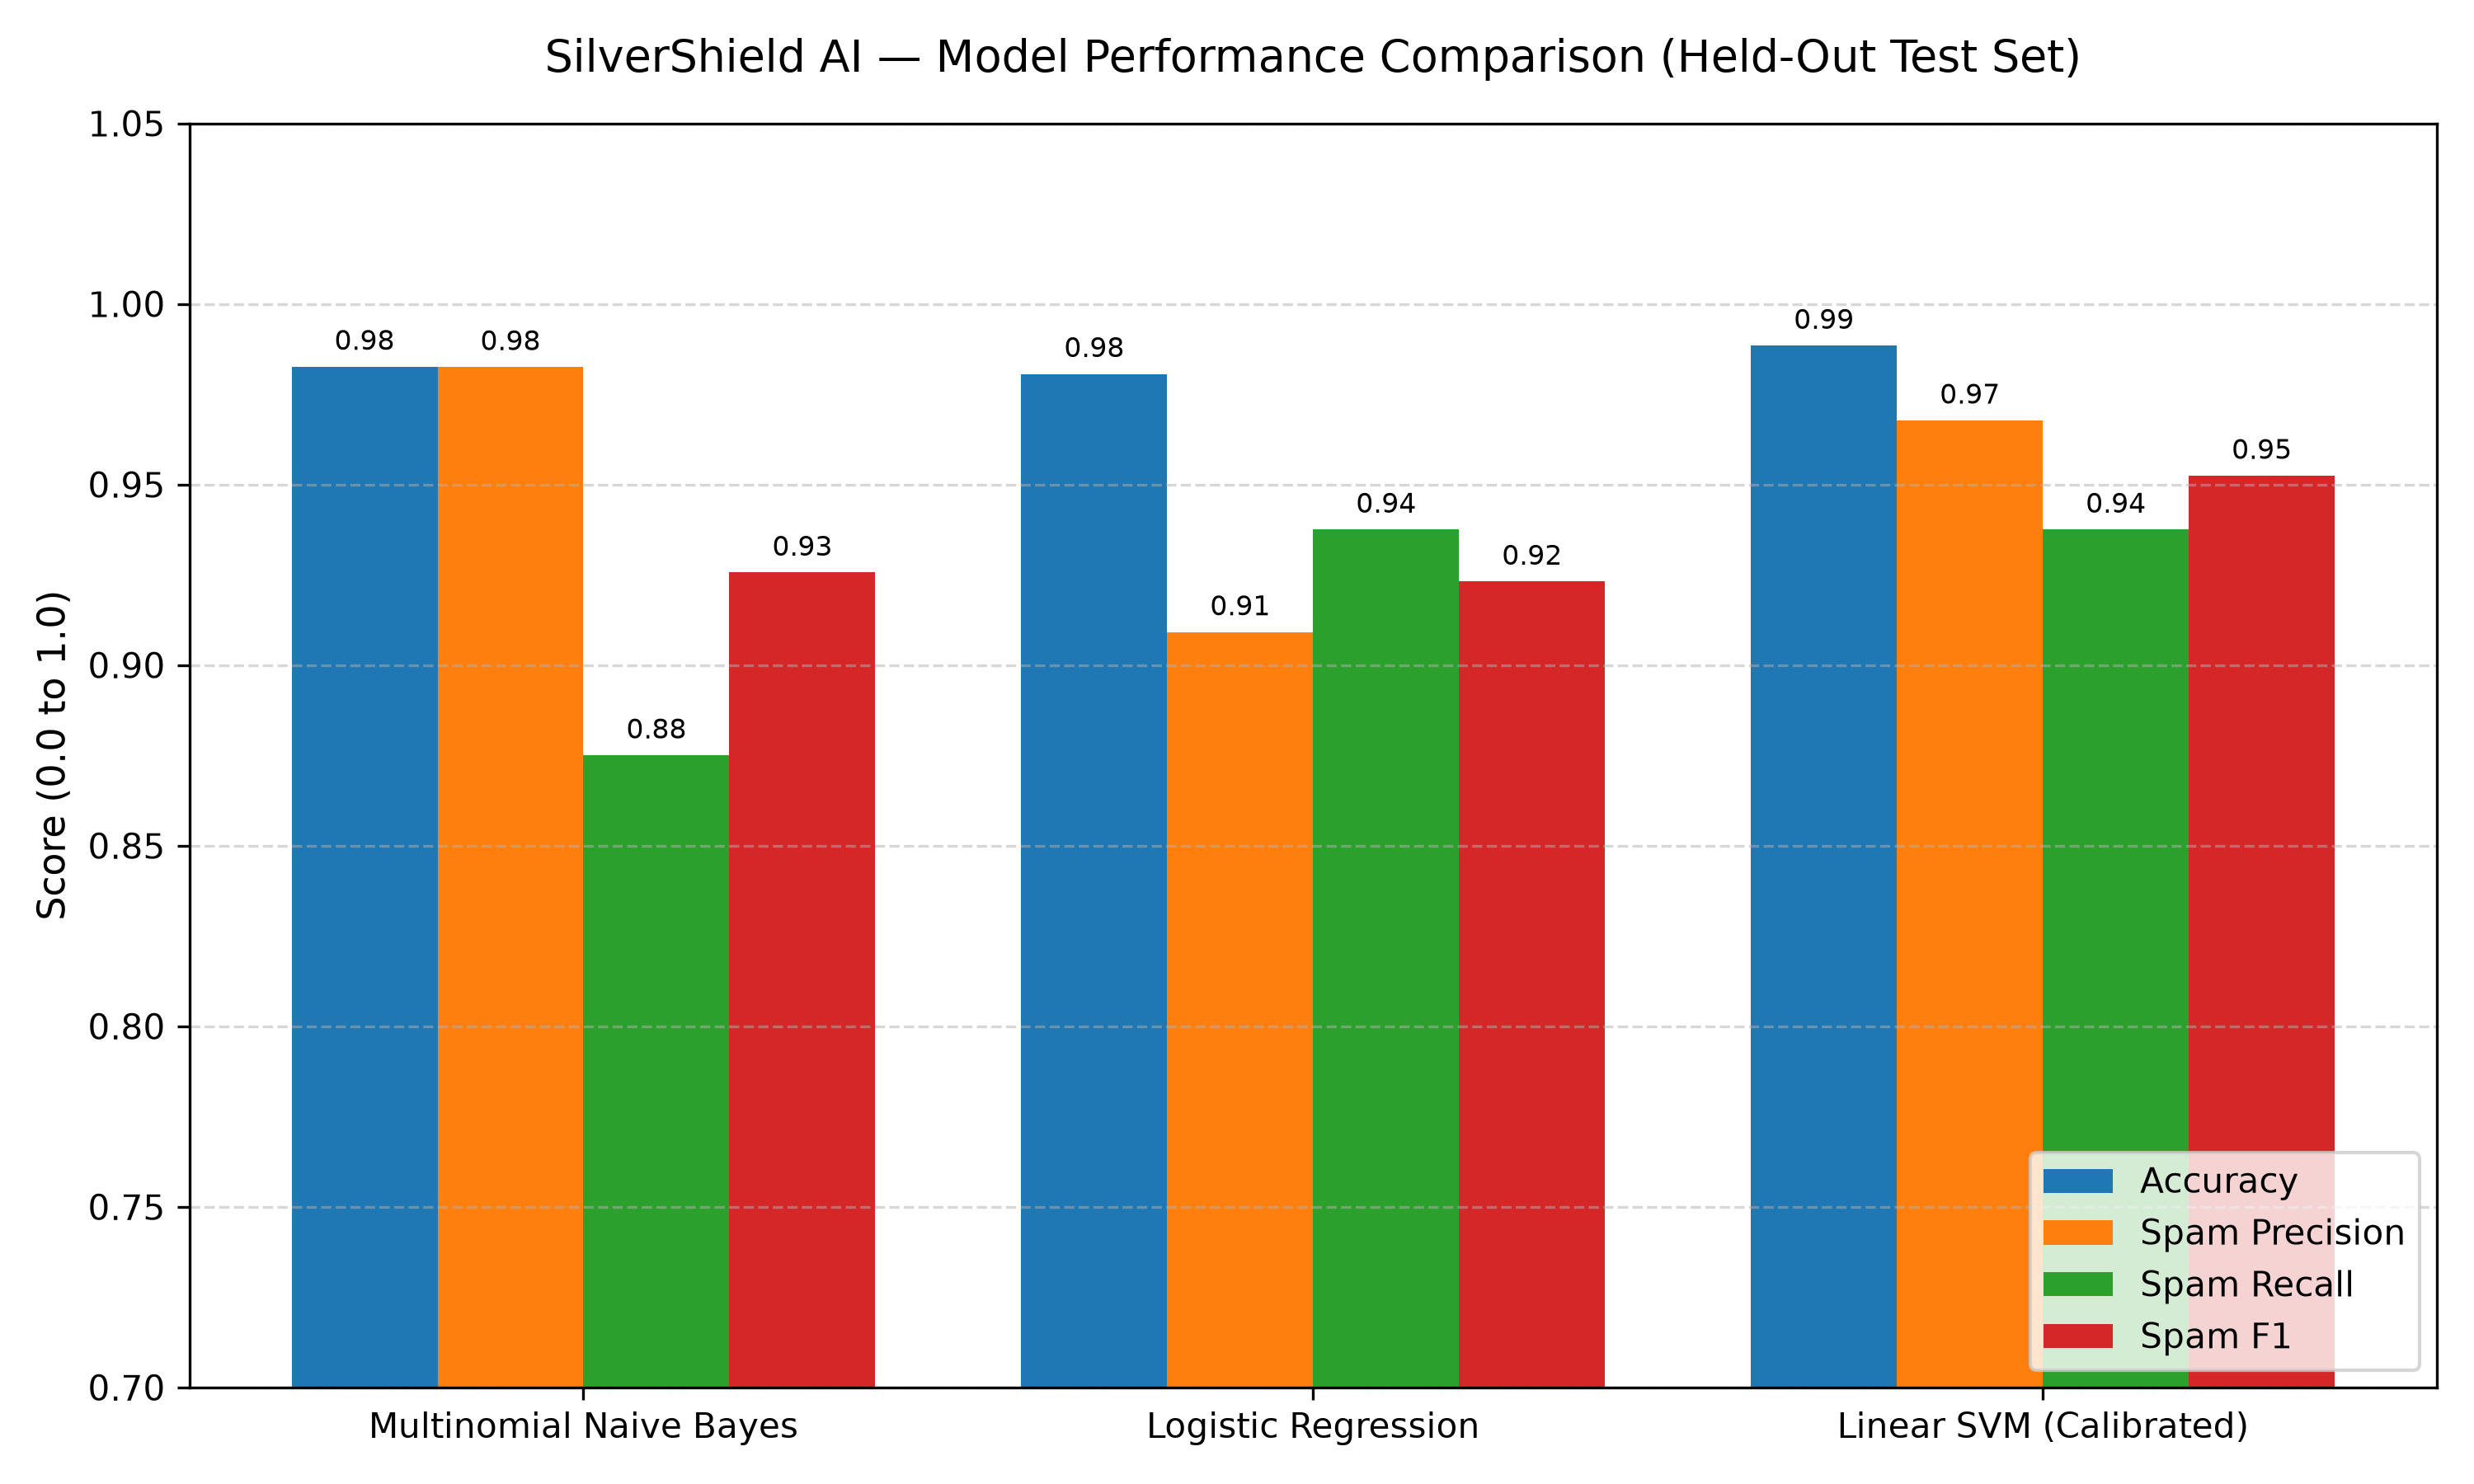
\includegraphics[width=\columnwidth]{images/model_comparison_chart.png}
\caption{Comparative performance metrics between Logistic Regression (Champion) and Multinomial Naive Bayes across Accuracy, Recall, Precision, and F1-Score.}
\label{fig:charts}
\end{figure}

Fig.~\ref{fig:cm_roc} displays the confusion matrix and Receiver Operating Characteristic (ROC) curve for the Champion Logistic Regression model.

\begin{figure}[t]
\centering
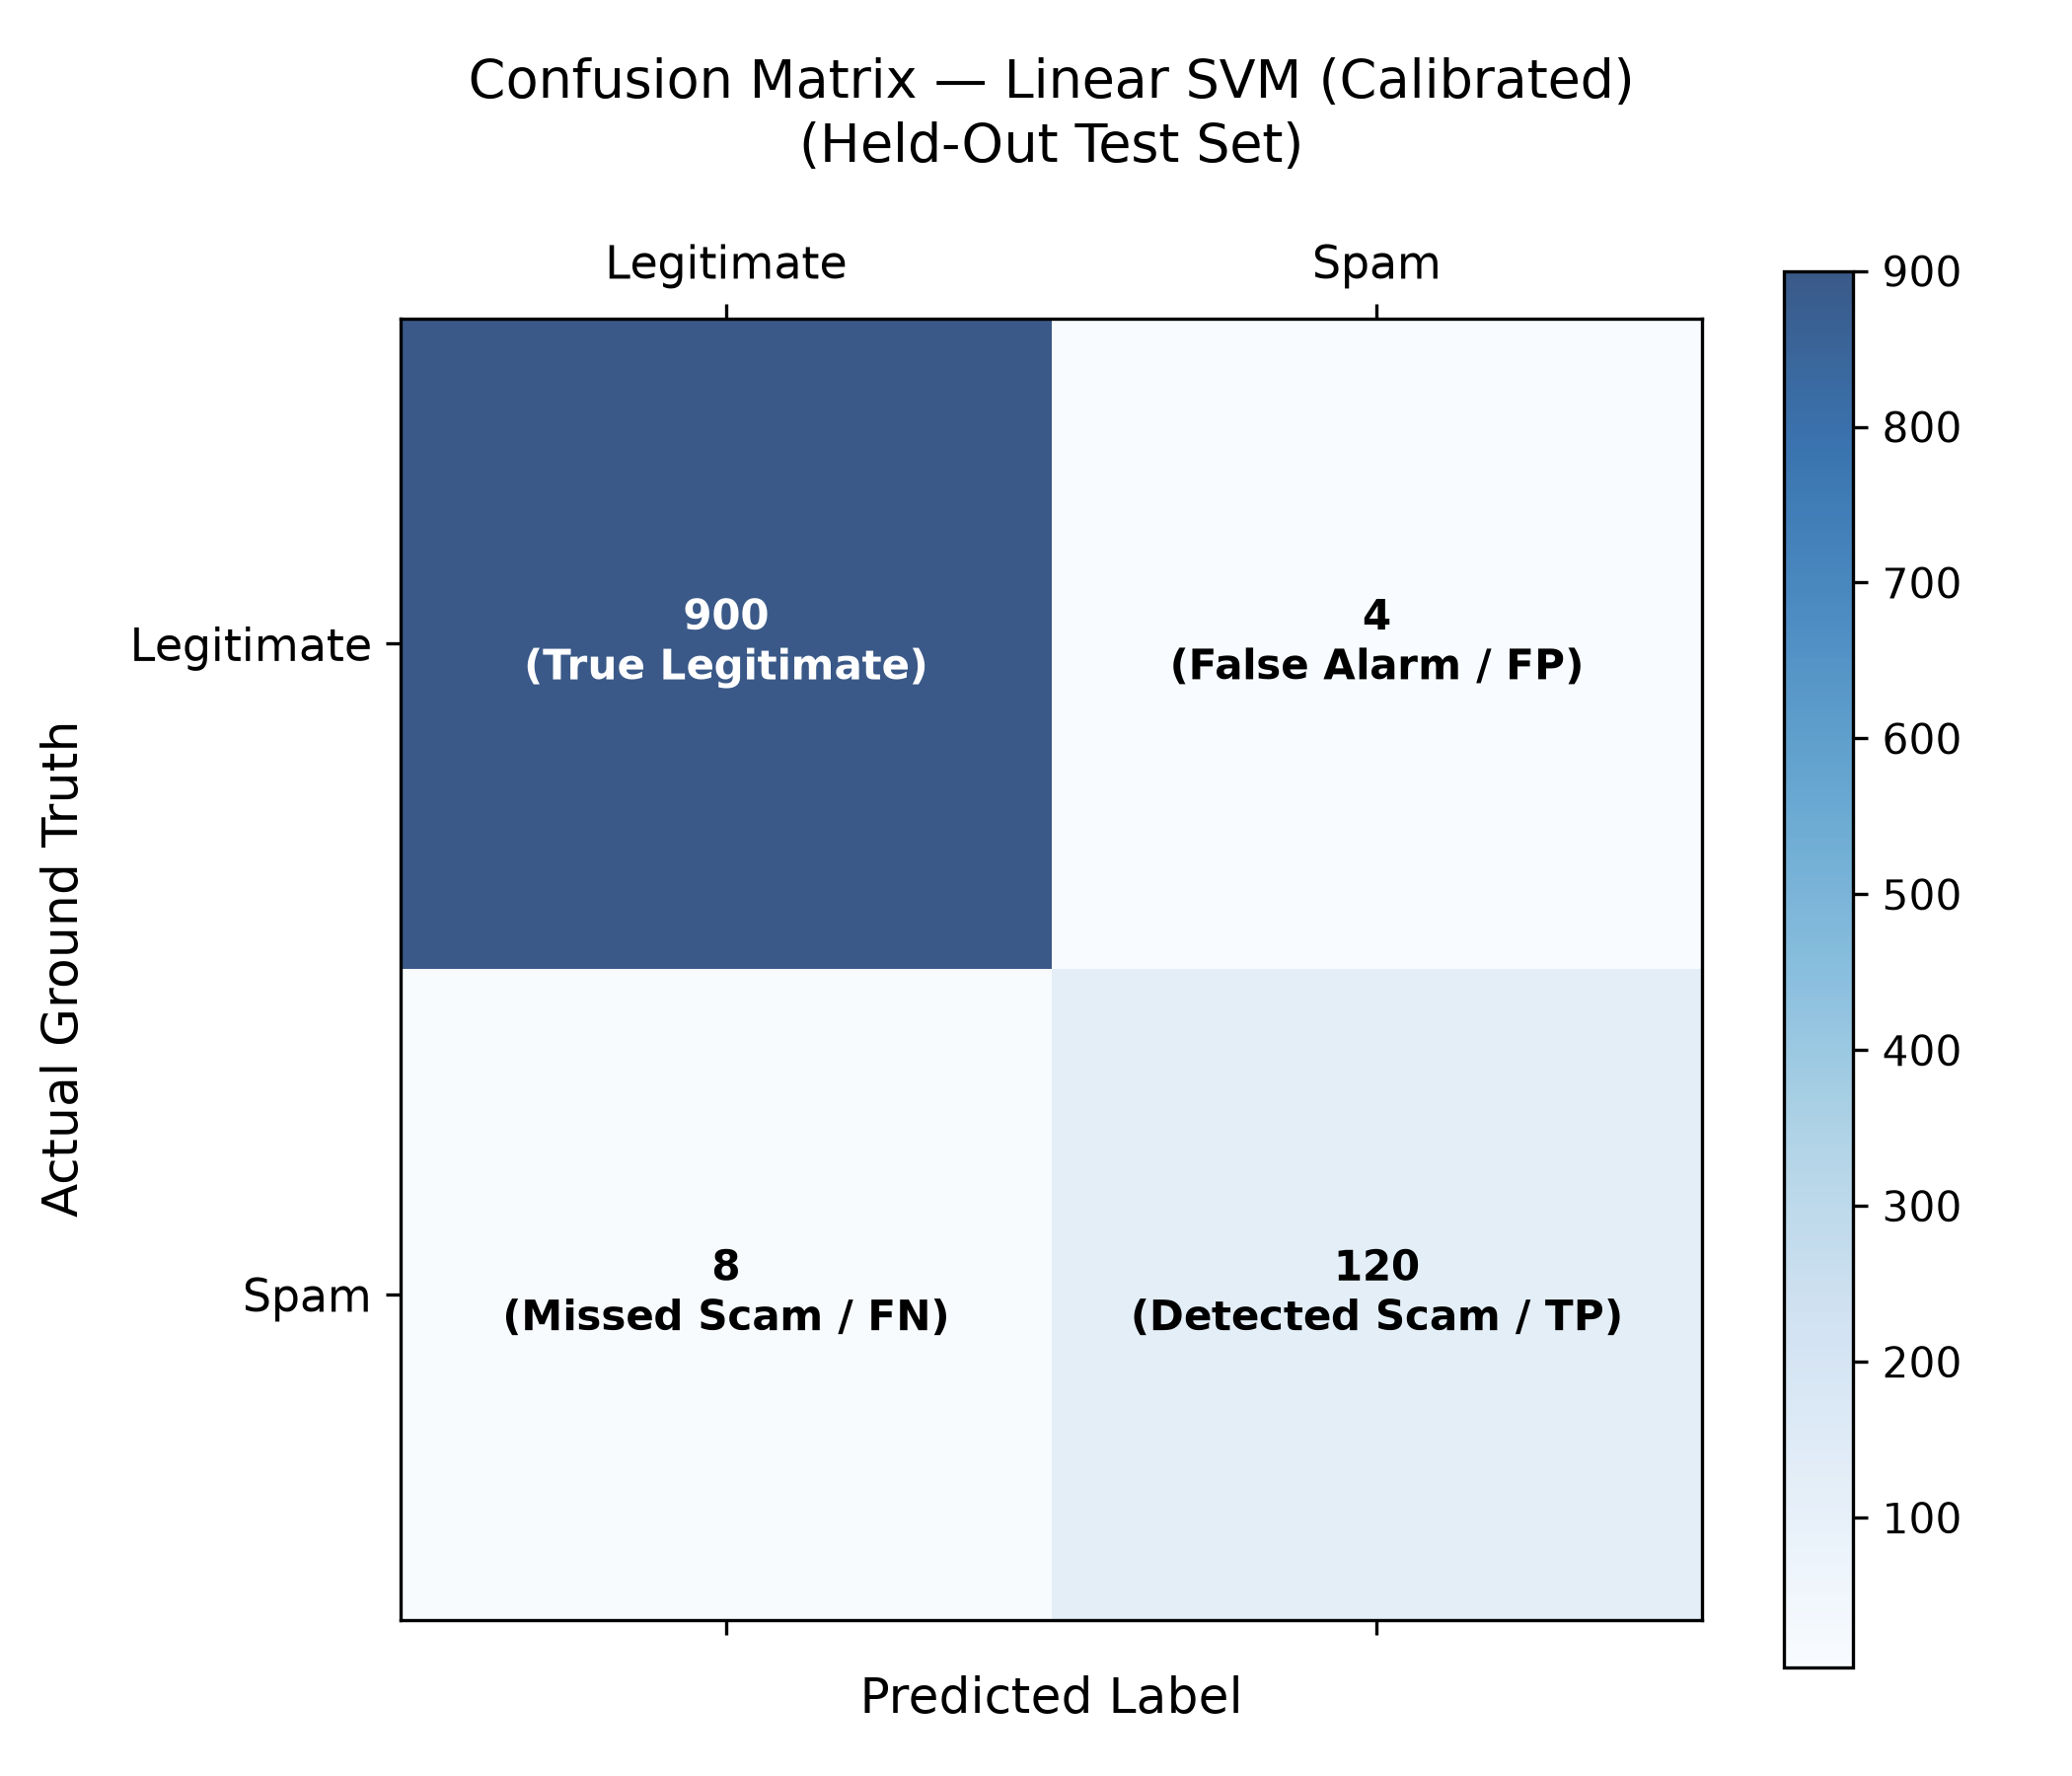
\includegraphics[width=0.48\columnwidth]{images/confusion_matrix.png}
\hfill
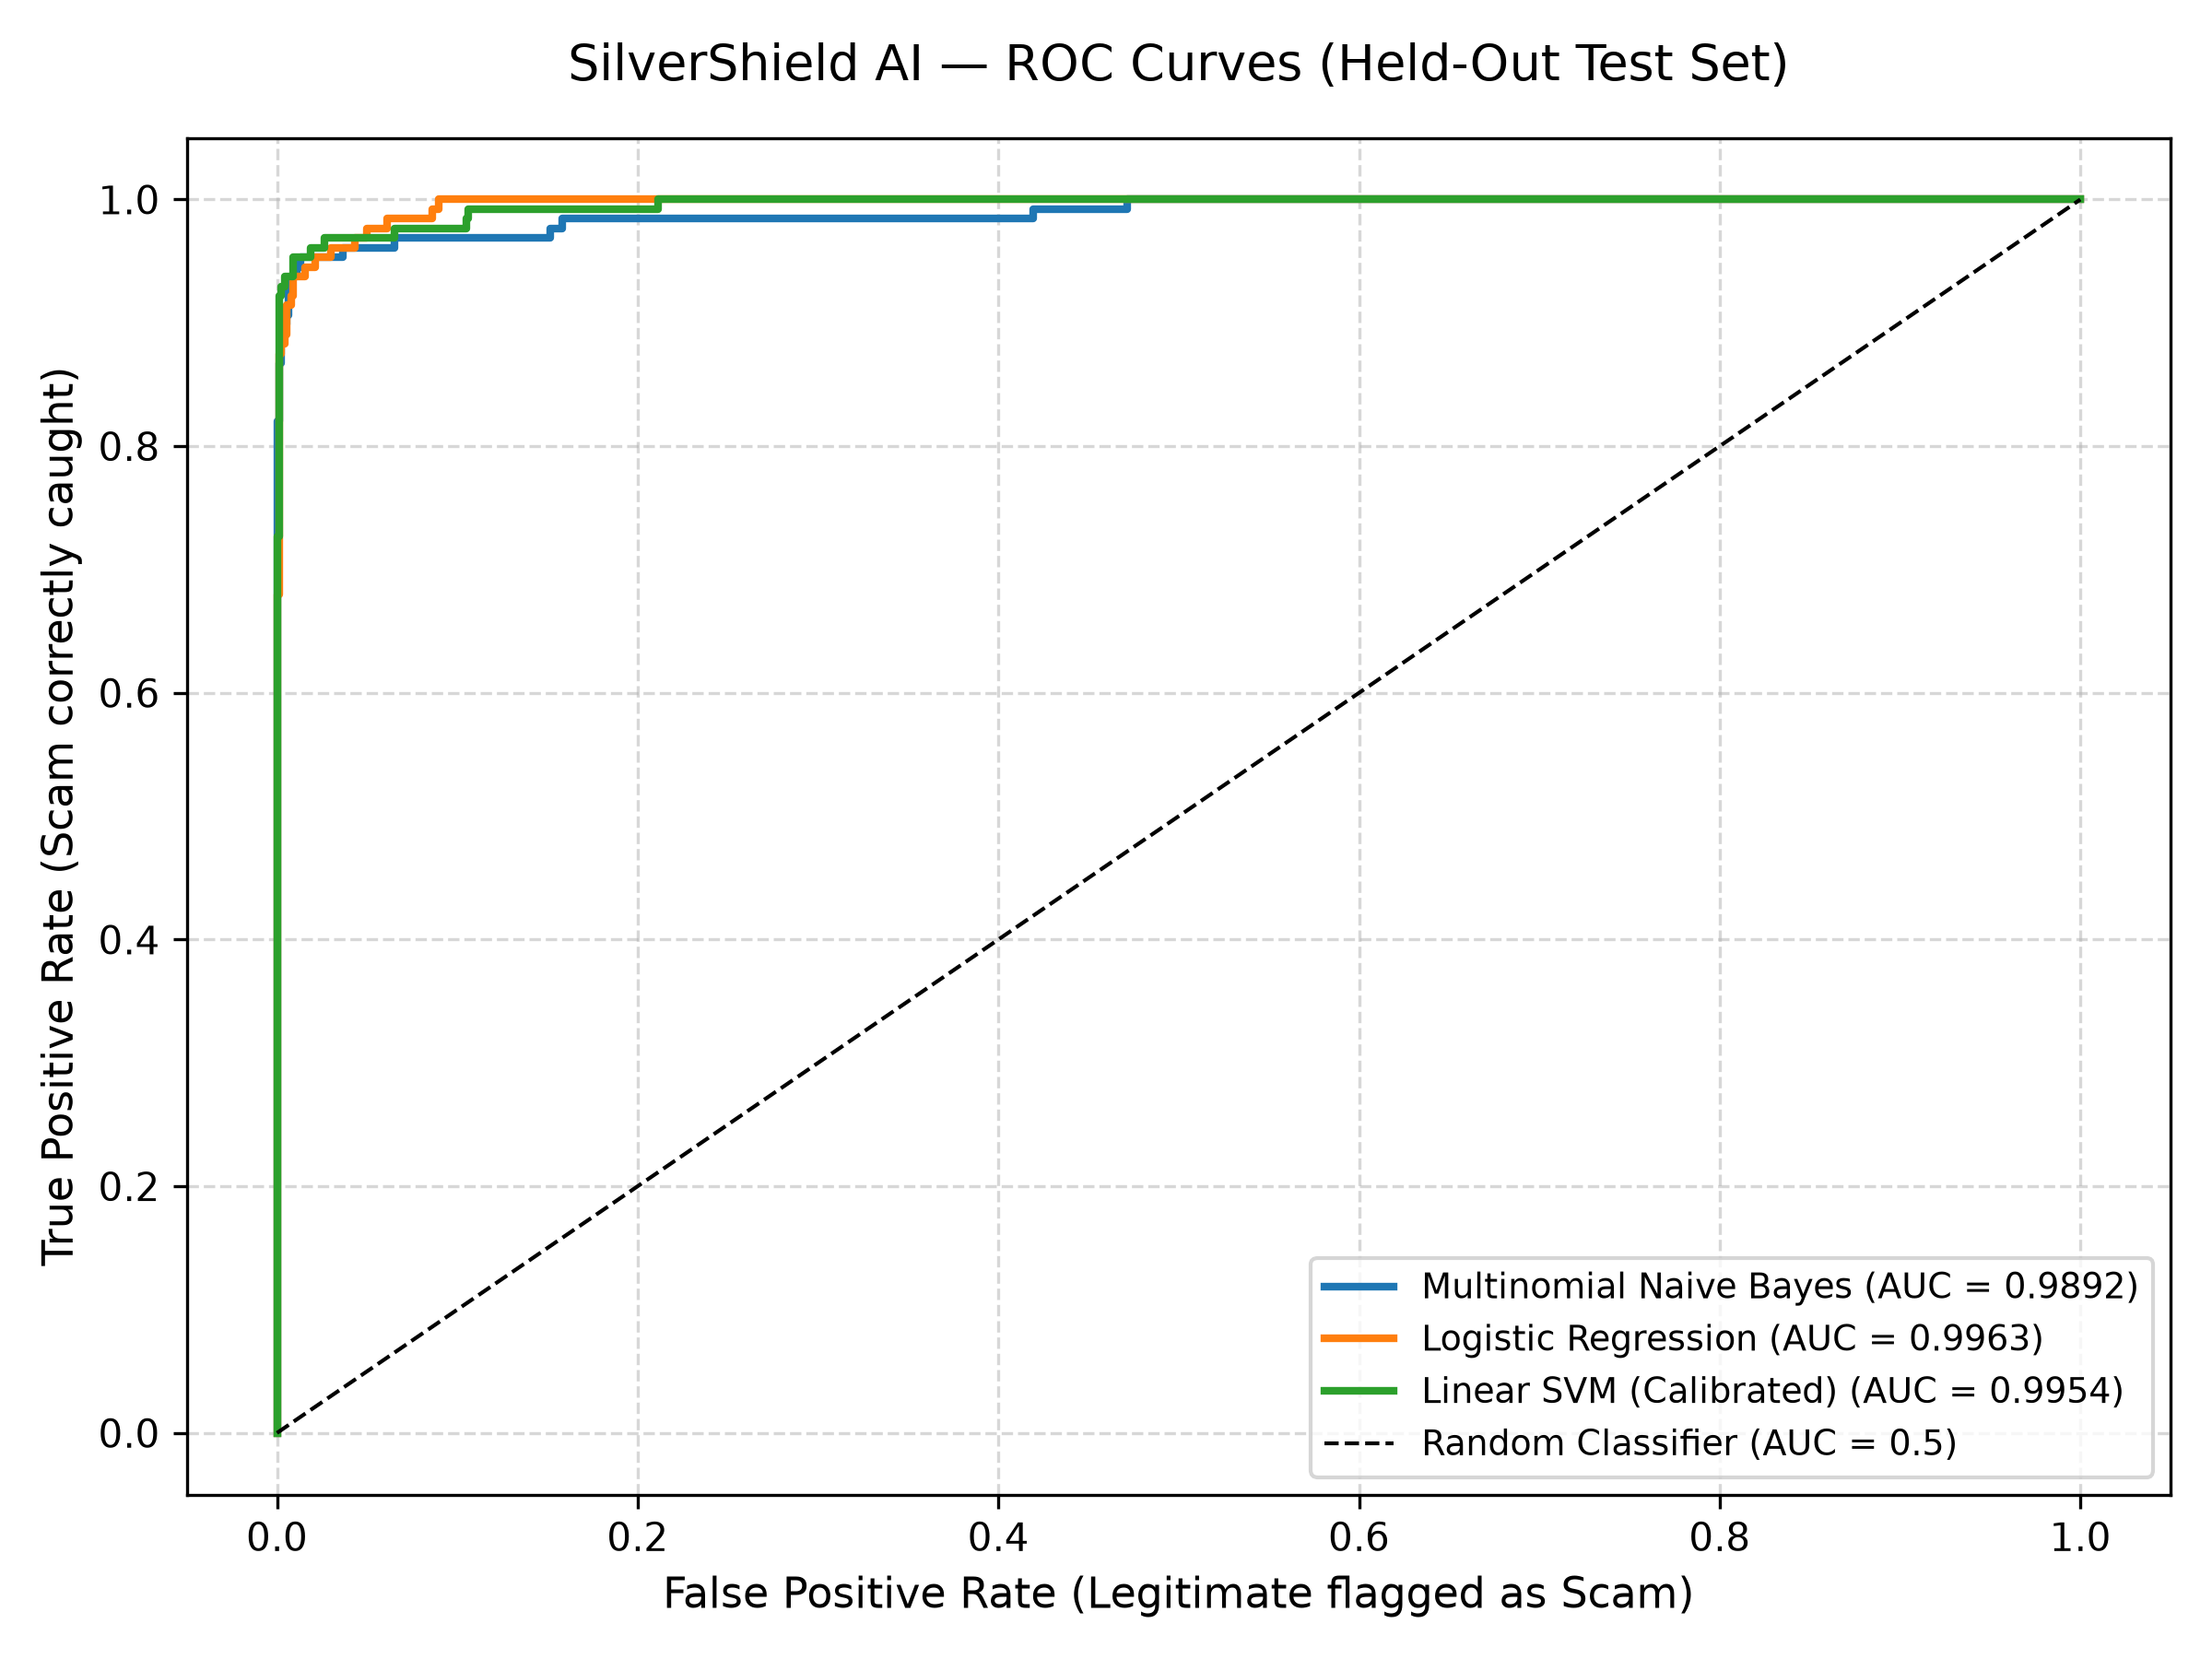
\includegraphics[width=0.48\columnwidth]{images/roc_curve.png}
\caption{Evaluation plots for Logistic Regression: (Left) Confusion Matrix showing 892 TN, 12 FP, 8 FN, 120 TP; (Right) ROC Curve illustrating near-ideal separation with $\text{AUC} = 0.9963$.}
\label{fig:cm_roc}
\end{figure}

\subsection{URL Analysis Verification}
The 9 heuristic inspection layers were validated against a benchmark battery of deceptive URLs, shown in Table~\ref{tab:url_tests}. In all scenarios, query strings were successfully sanitized prior to output.

\begin{table}[h]
\caption{URL Analysis Heuristic Verification Results}
\label{tab:url_tests}
\centering
\small
\begin{tabular}{lp{3.5cm}r}
\toprule
\textbf{Target Test URL} & \textbf{Triggered Heuristic Flags} & \textbf{Verdict} \\
\midrule
\texttt{http://192.168.1.5/login} & IP Address Host, Credential Path & MALICIOUS \\
\texttt{https://bit.ly/sbi-kyc} & URL Shortener, Suspicious Keywords & SUSPICIOUS \\
\texttt{http://sbi.verify.xyz} & High-Risk TLD (.xyz), Subdomain Depth & MALICIOUS \\
\texttt{https://g00gle.com/secure} & Brand Homoglyph, Path Keyword & SUSPICIOUS \\
\texttt{https://google.com/search} & None (Legitimate domain) & SAFE \\
\bottomrule
\end{tabular}
\end{table}

\subsection{Functional Testing Suite}
The system implementation was verified through an automated test suite comprising **162 passing tests** executed via Pytest. Table~\ref{tab:test_cases} highlights representative functional test scenarios.

\begin{table}[h]
\caption{Representative Functional Test Scenarios}
\label{tab:test_cases}
\centering
\small
\begin{tabular}{p{1.2cm}p{3.2cm}p{2.8cm}}
\toprule
\textbf{Test ID} & \textbf{Input Condition} & \textbf{Observed Output} \\
\midrule
TC-01 & Benign grocery arrival message & Overall Risk: LOW (0 pts), routine advice \\
TC-02 & Urgent bank block alert + OTP & Overall Risk: HIGH (OVR-01, OVR-03) \\
TC-03 & Delivery notice with shortened link & Overall Risk: MEDIUM (URL Shortener) \\
TC-04 & OTP request + external login URL & Forced HIGH via OVR-03 \\
TC-05 & ML microservice connection timeout & Graceful degradation: MEDIUM floor \\
TC-06 & Access to \texttt{/auth/me} without JWT & HTTP 401 Unauthorized \\
TC-07 & 20 rapid login attempts from same IP & HTTP 429 Rate Limit Exceeded \\
TC-08 & Non-existent email login attempt & Dummy Argon2id timing defense \\
\bottomrule
\end{tabular}
\end{table}

\subsection{Application Interface Walkthrough}
The application interface provides an intuitive experience designed specifically for senior citizens. Fig.~\ref{fig:ui_screens} showcases representative views of the implemented system.

\begin{figure*}[t]
\centering
\begin{minipage}{0.32\textwidth}
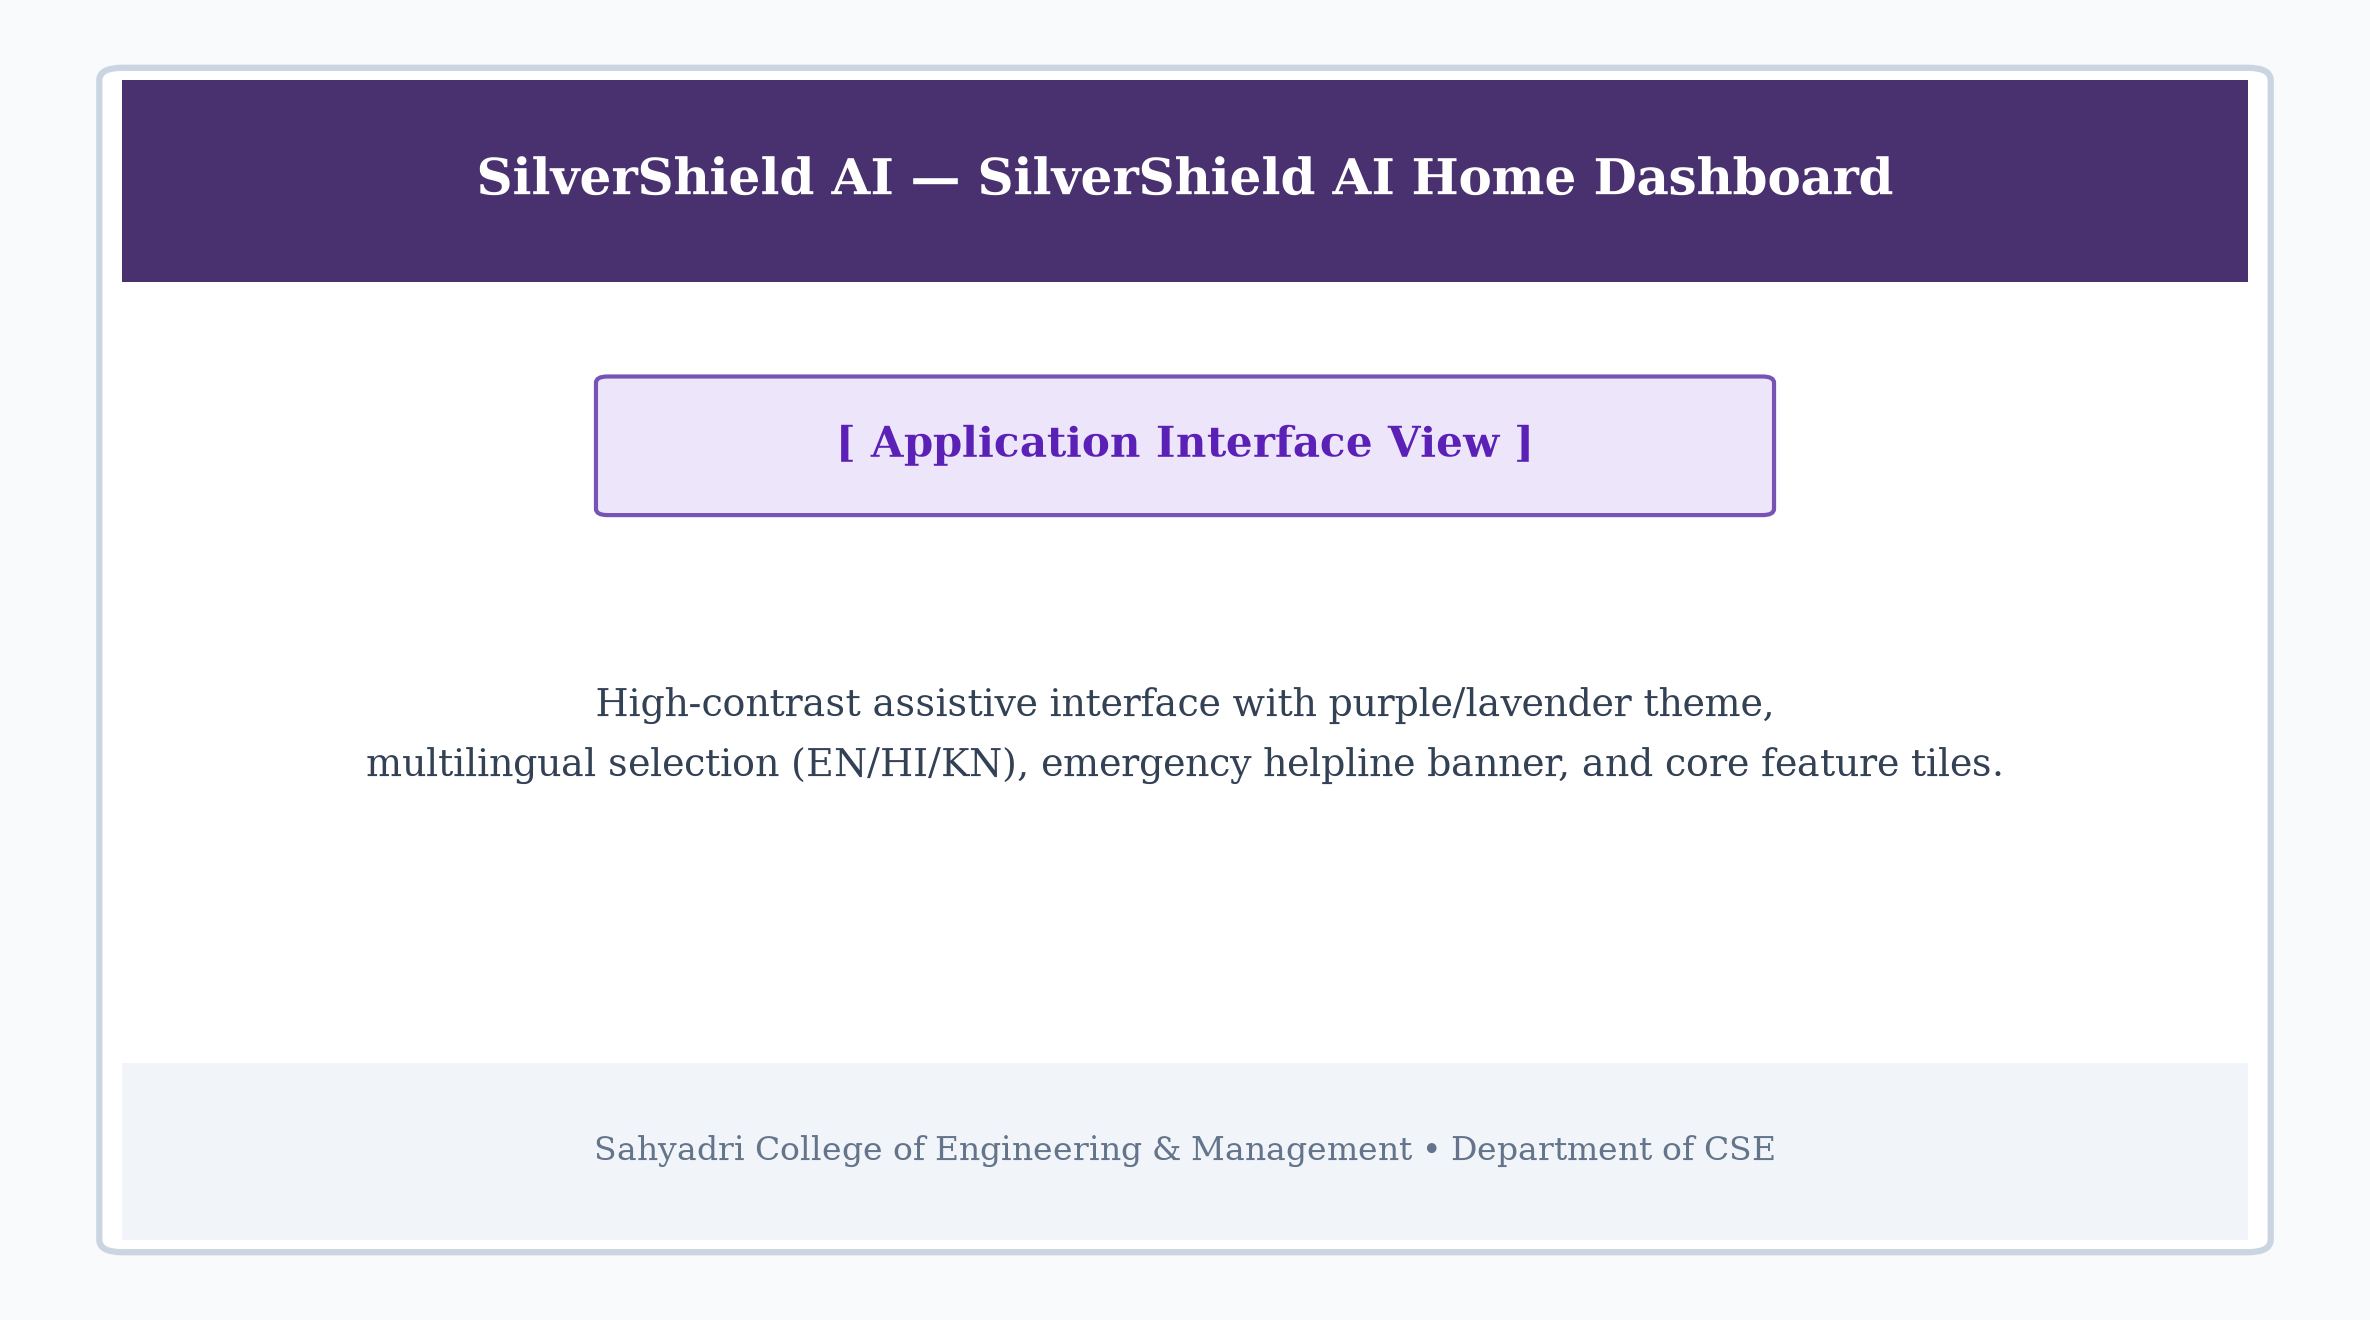
\includegraphics[width=\textwidth]{images/ui_dashboard.png}
\centerline{\footnotesize (a) Home Dashboard \& Helpline Banner}
\end{minipage}
\hfill
\begin{minipage}{0.32\textwidth}
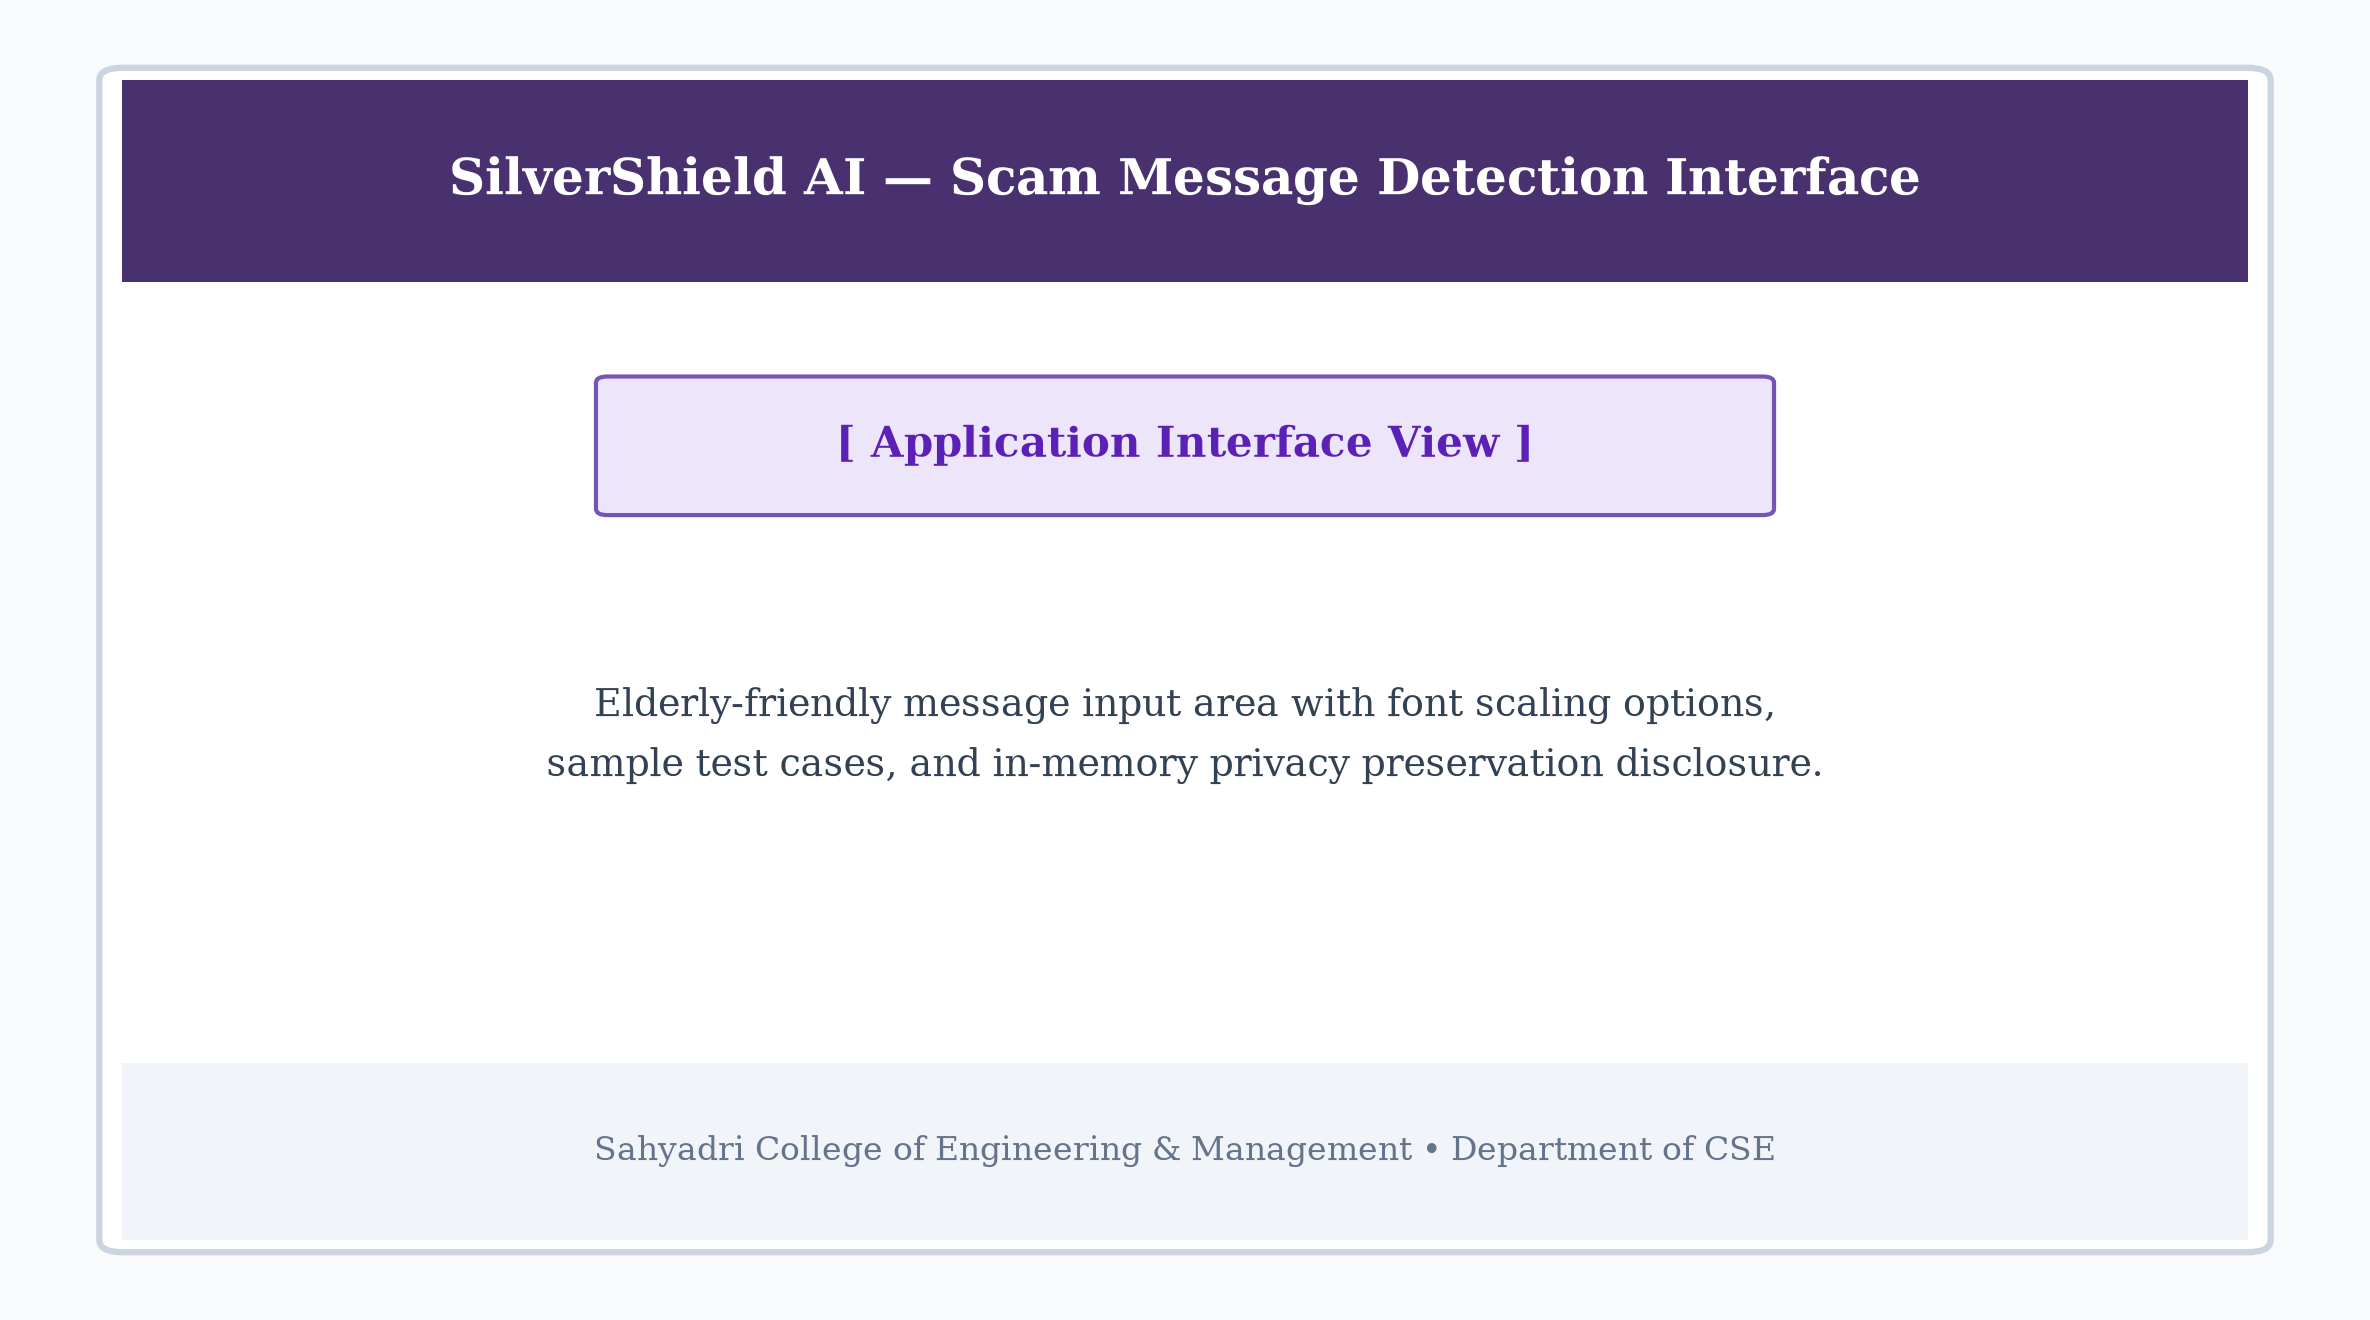
\includegraphics[width=\textwidth]{images/ui_scam_detector.png}
\centerline{\footnotesize (b) Scam Message Detection Input}
\end{minipage}
\hfill
\begin{minipage}{0.32\textwidth}
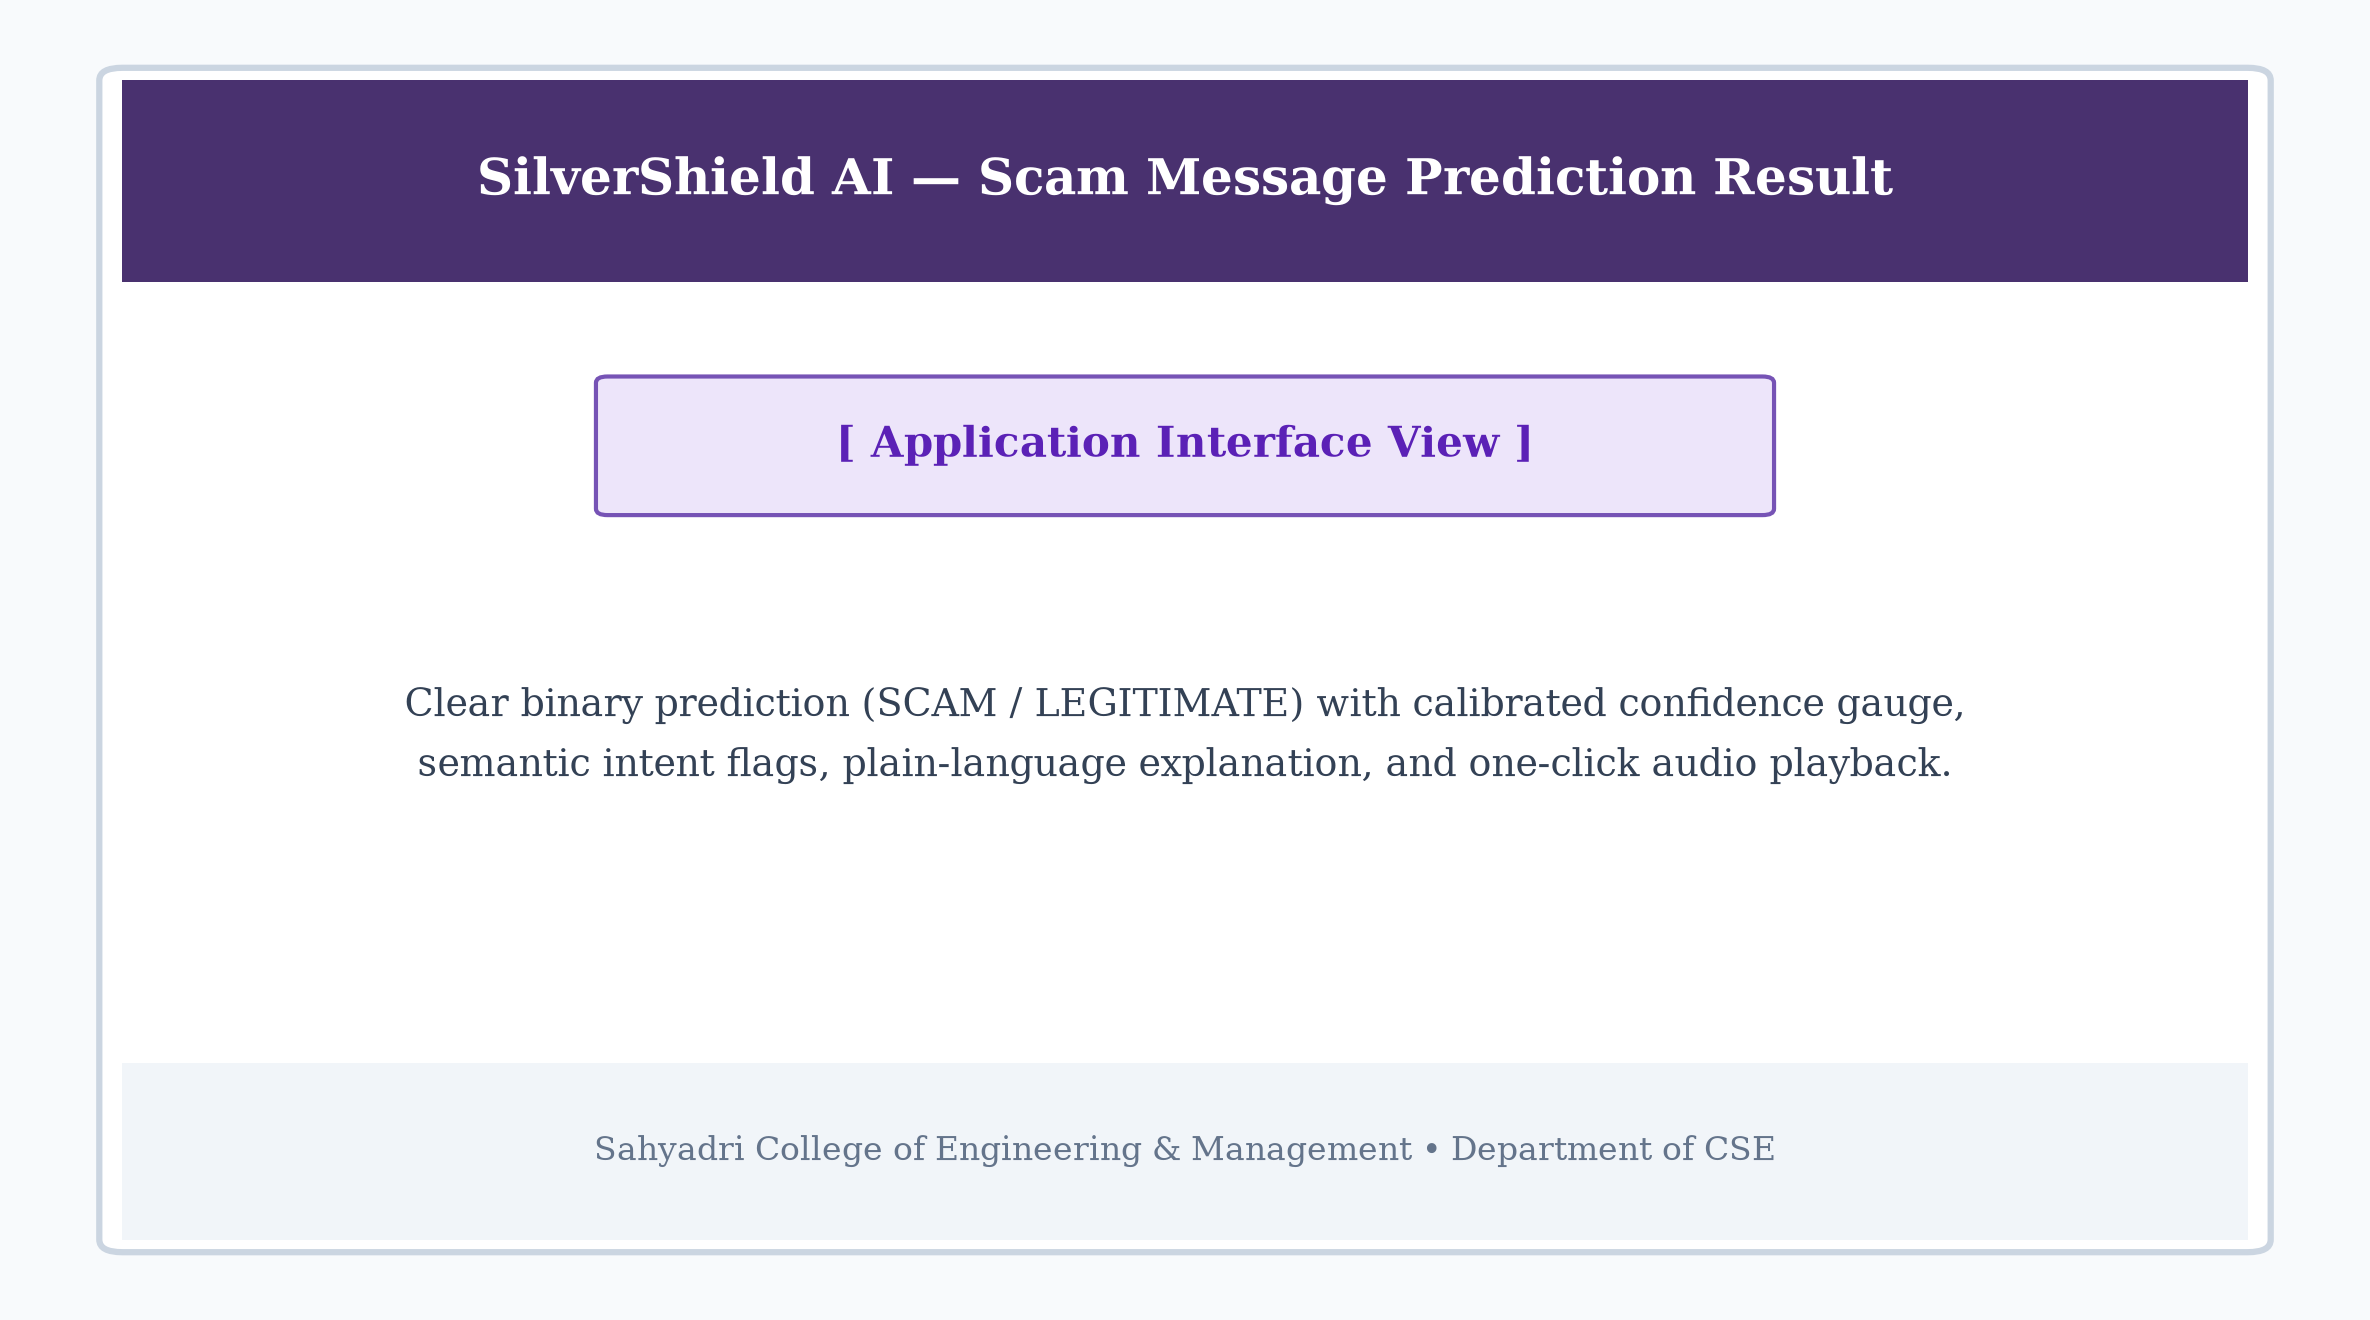
\includegraphics[width=\textwidth]{images/ui_scam_result.png}
\centerline{\footnotesize (c) Prediction Result \& Voice Narrator}
\end{minipage}
\par\vspace{2mm}
\begin{minipage}{0.32\textwidth}
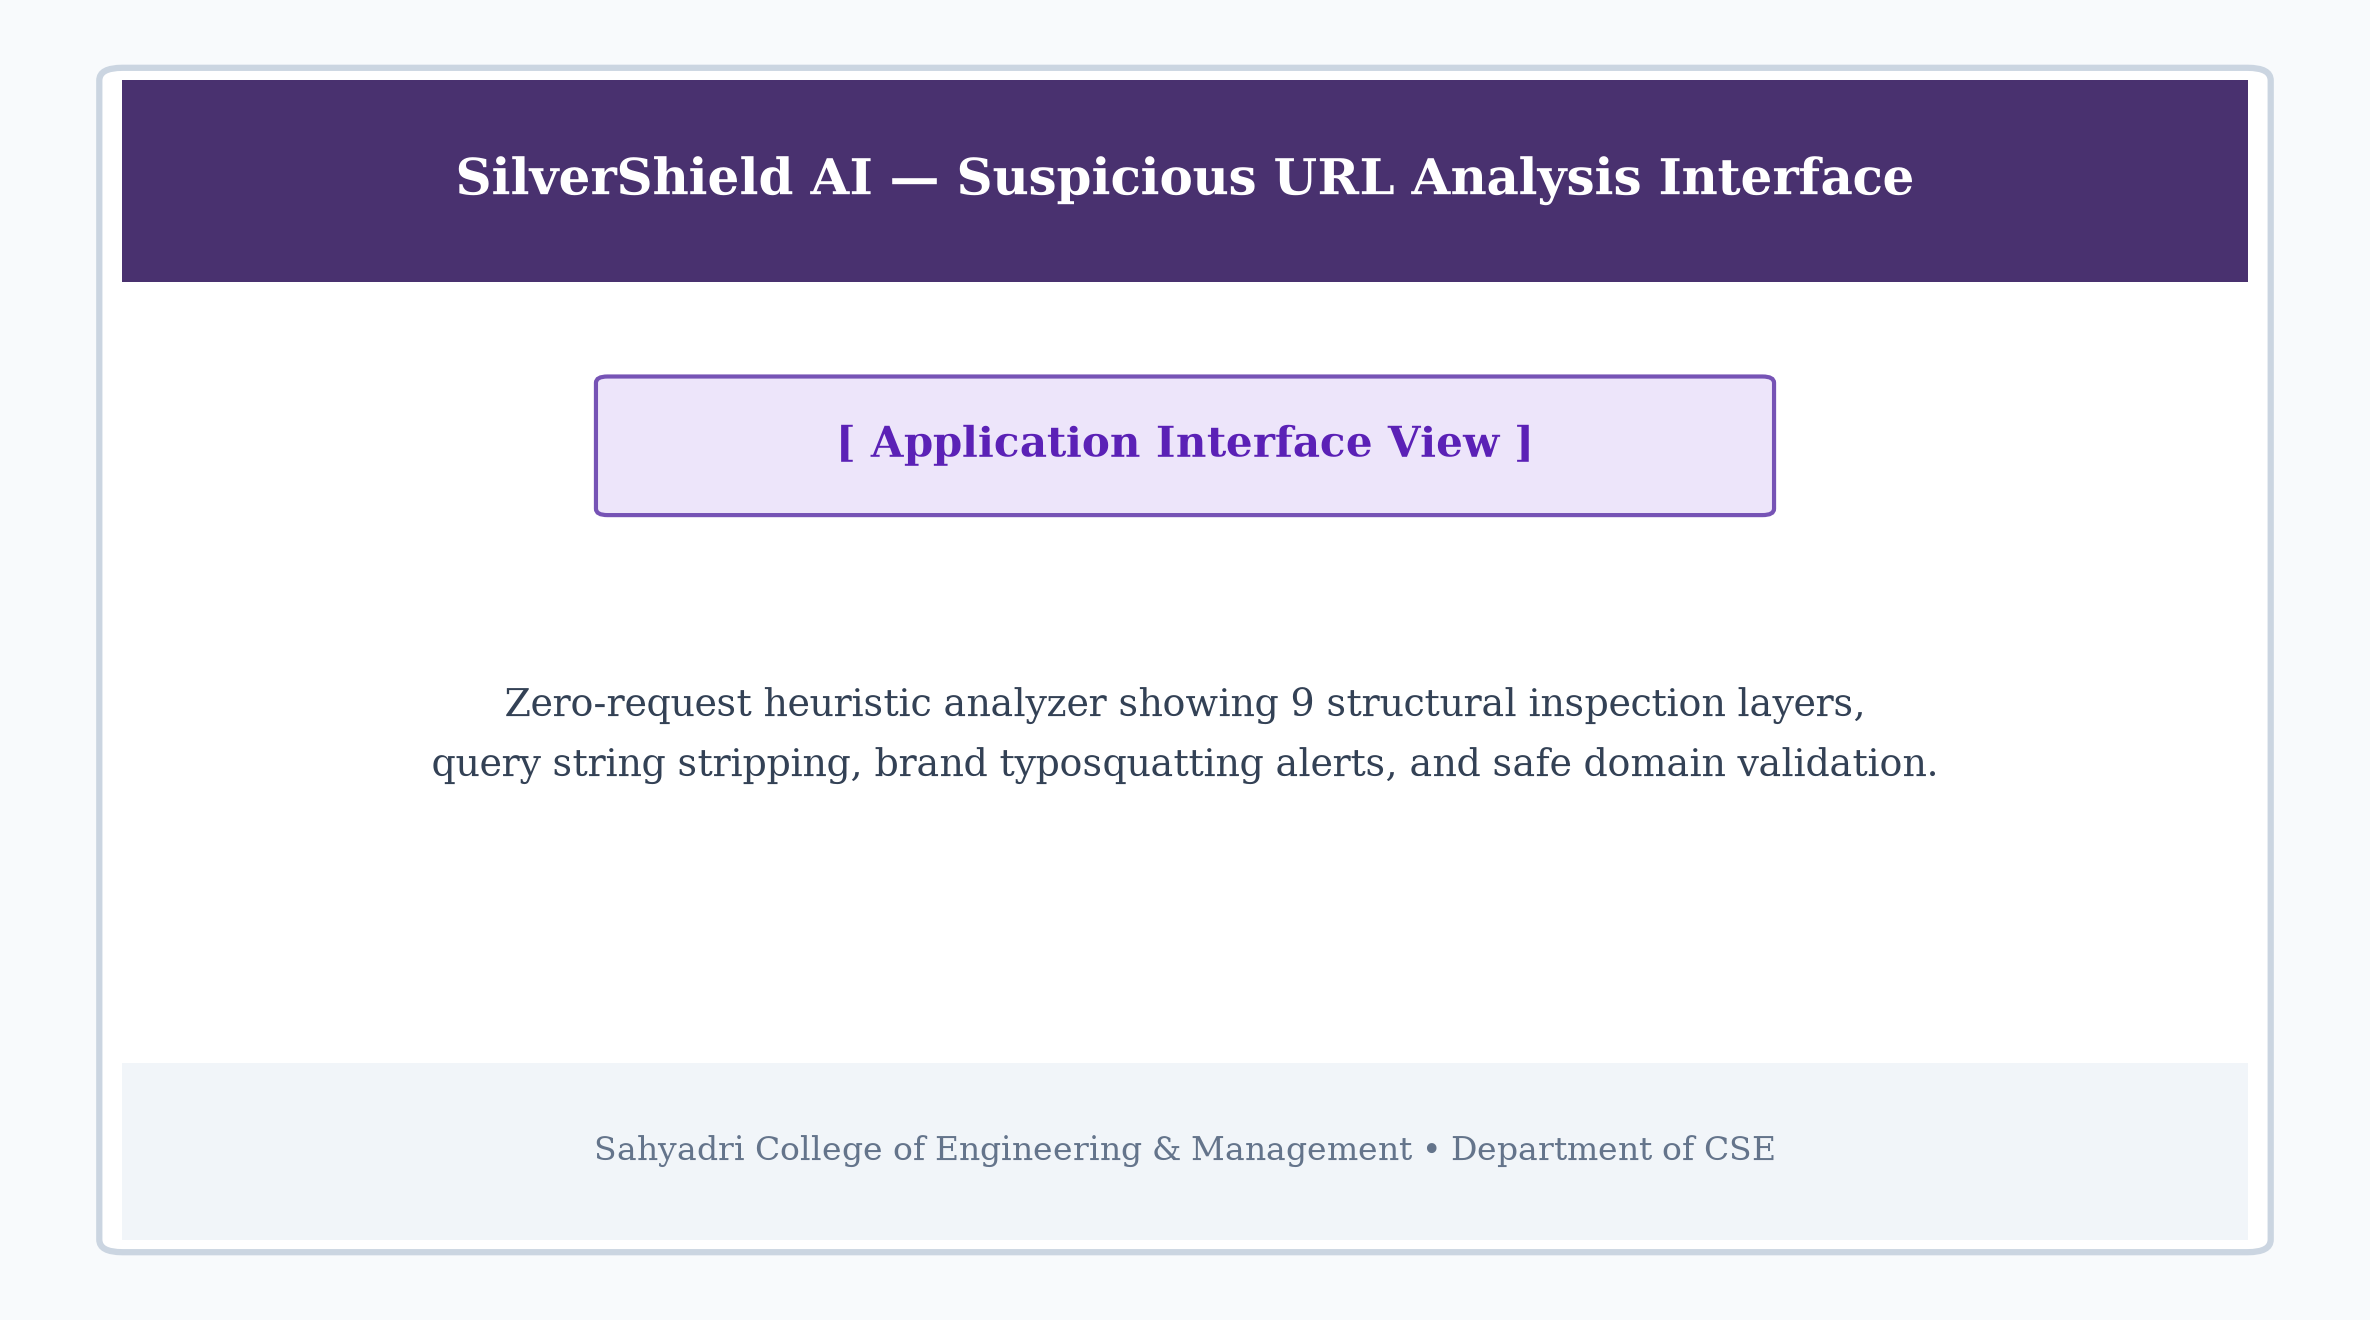
\includegraphics[width=\textwidth]{images/ui_url_analysis.png}
\centerline{\footnotesize (d) 9-Layer URL Security Inspection}
\end{minipage}
\hfill
\begin{minipage}{0.32\textwidth}
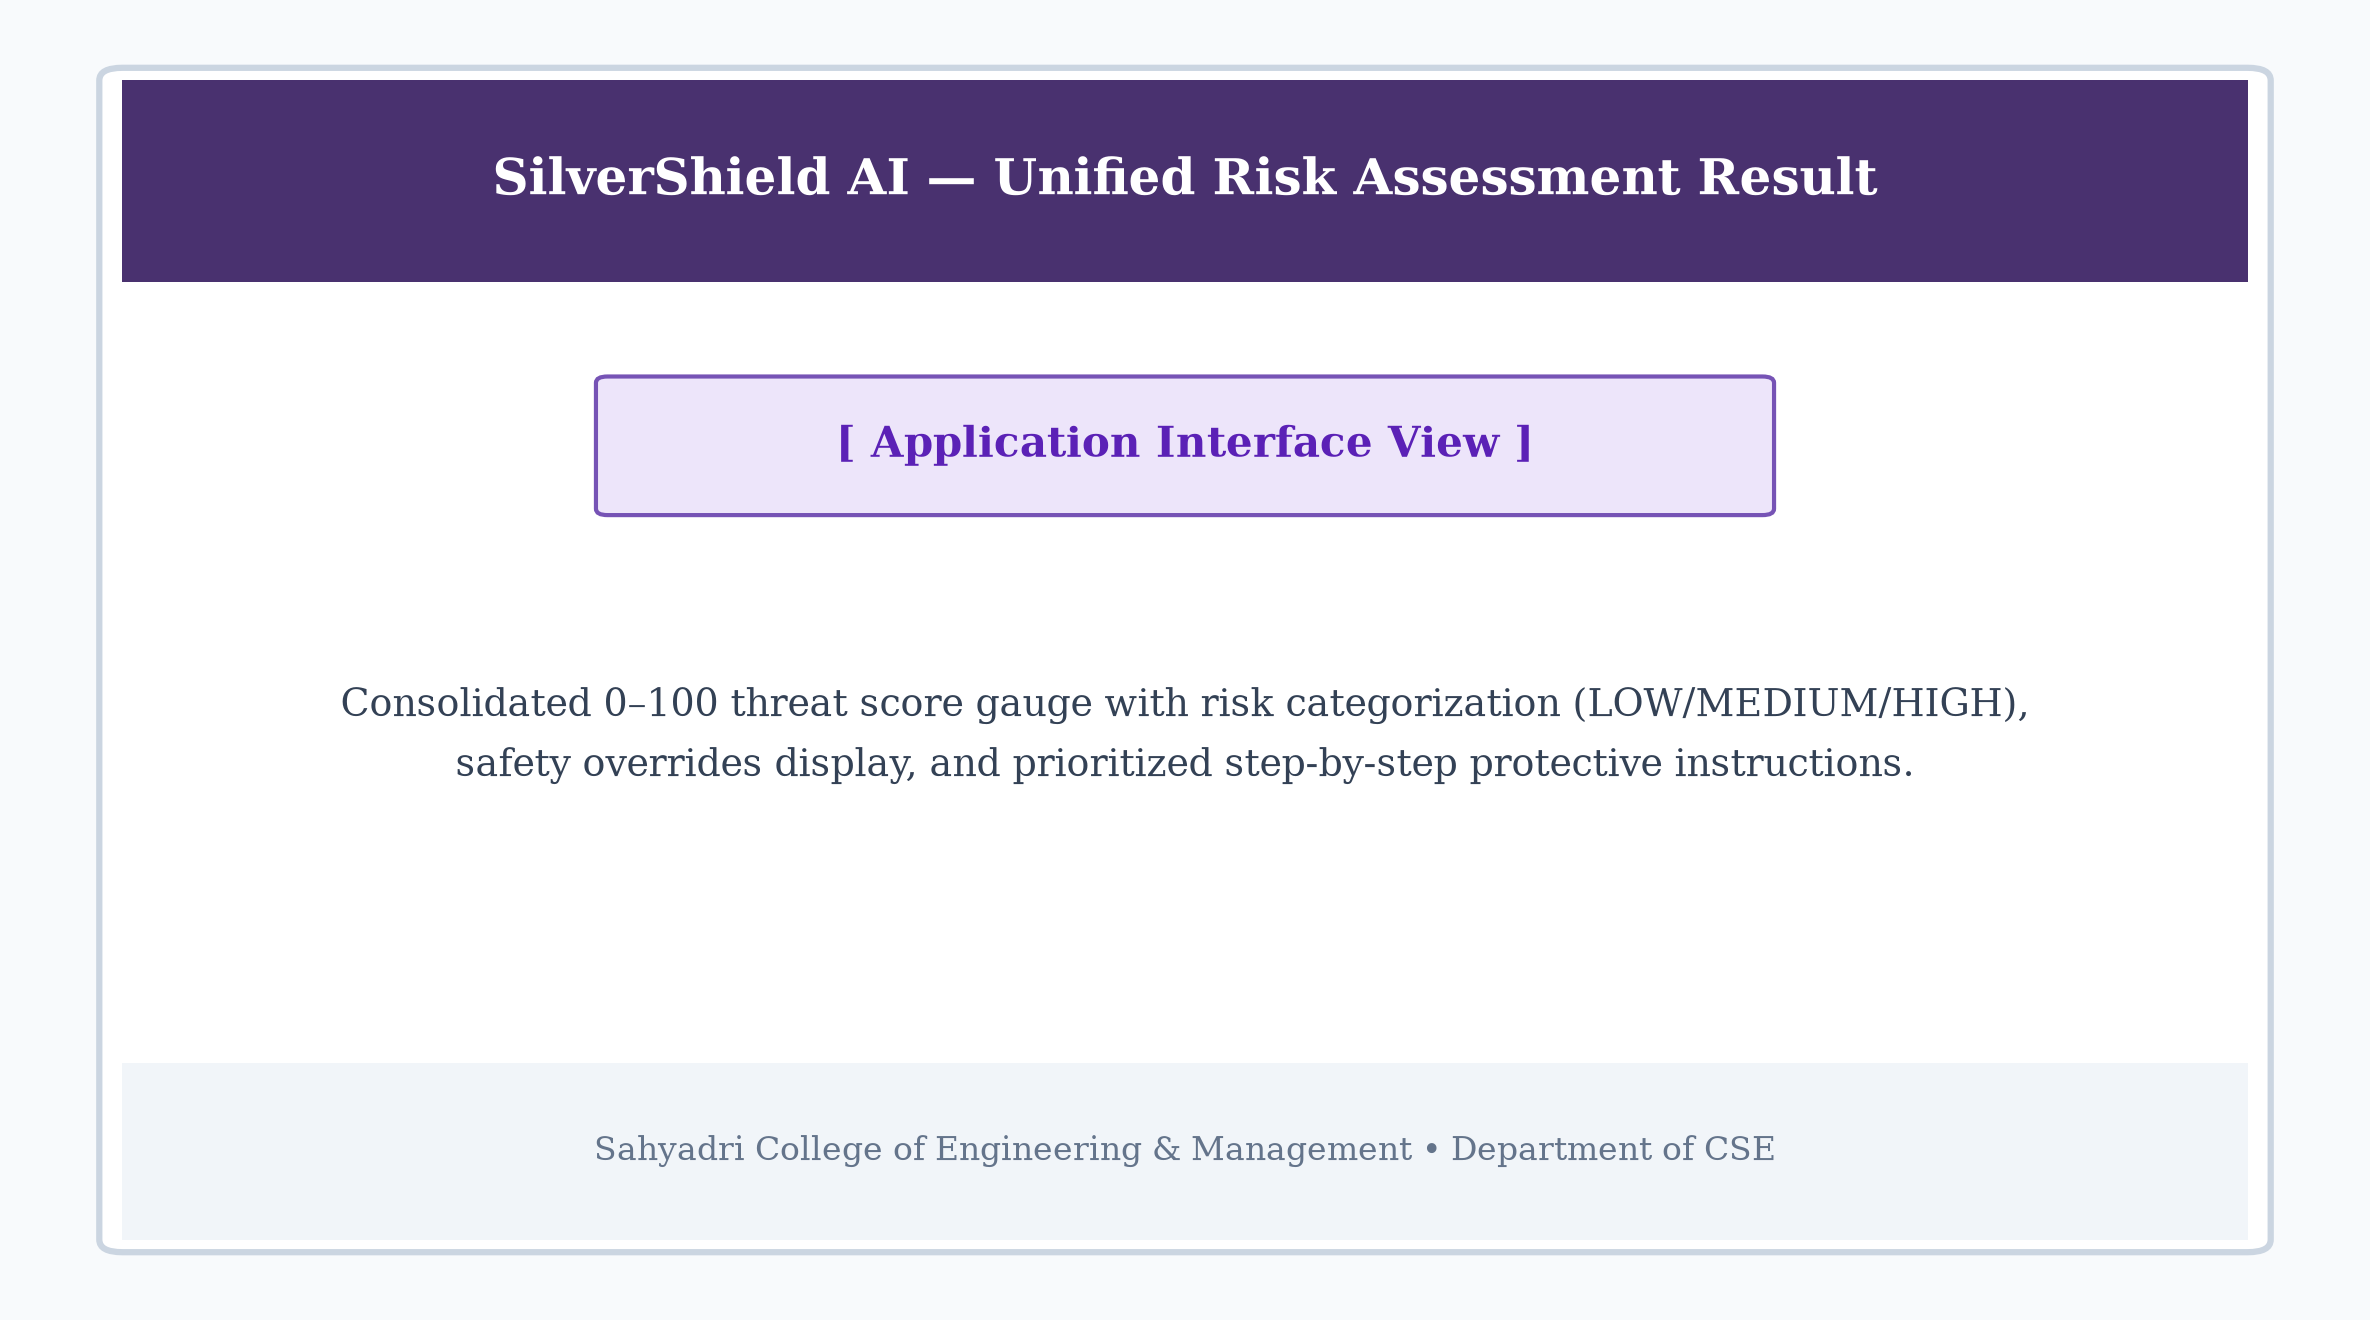
\includegraphics[width=\textwidth]{images/ui_risk_assessment.png}
\centerline{\footnotesize (e) Unified Risk Score \& Actions}
\end{minipage}
\hfill
\begin{minipage}{0.32\textwidth}
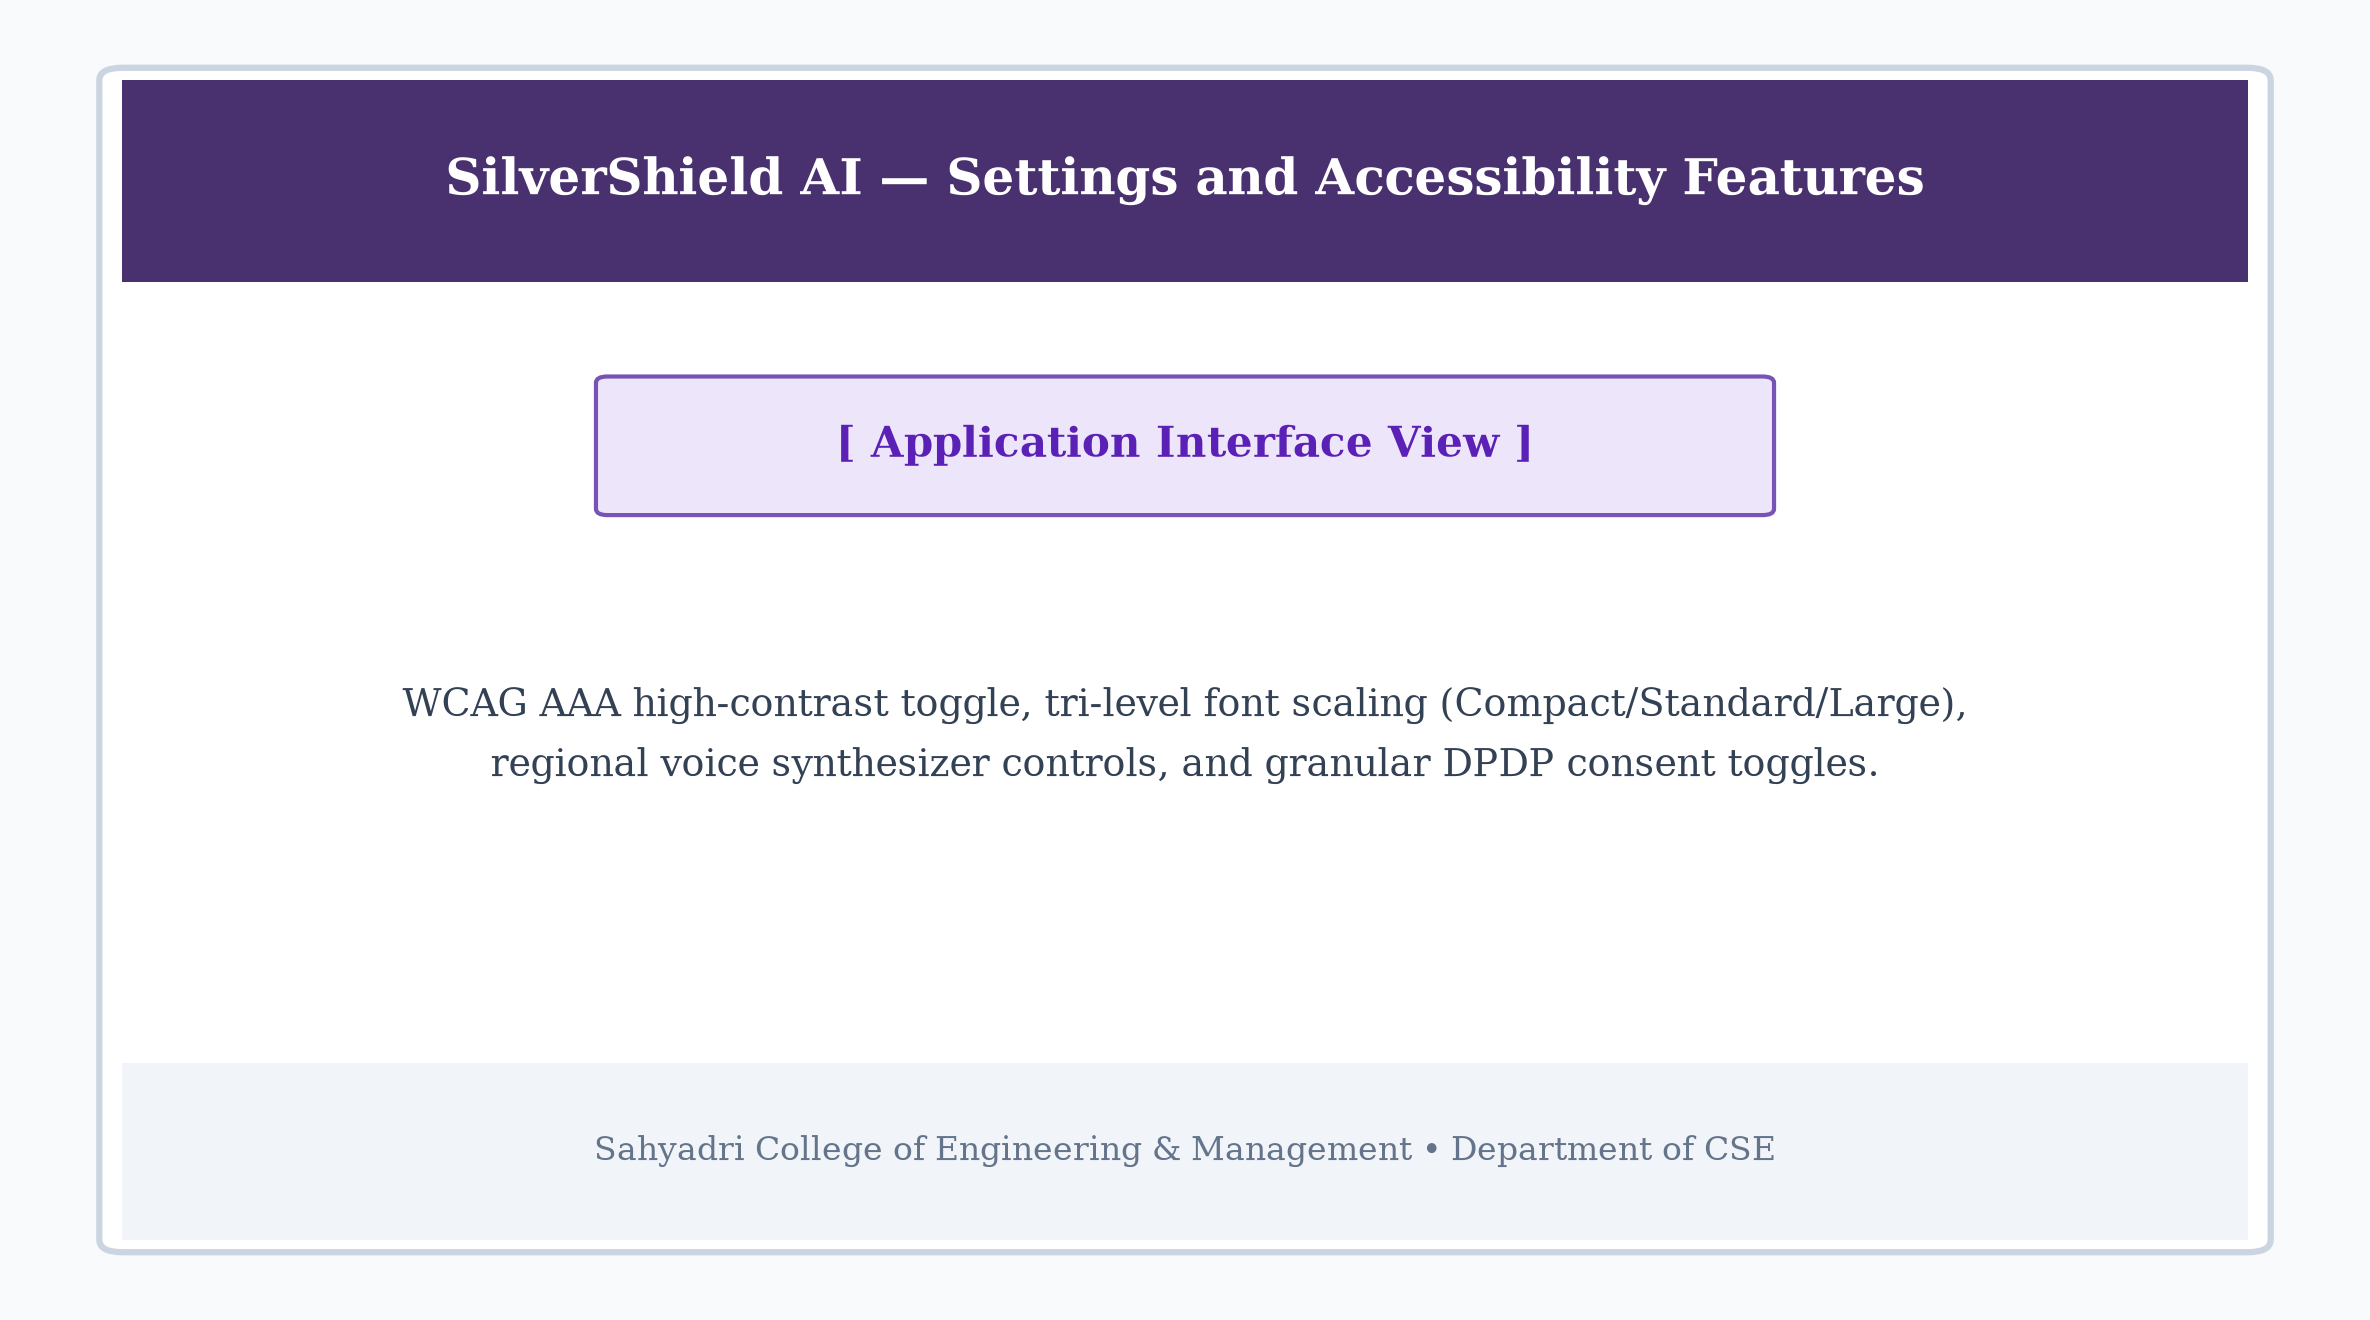
\includegraphics[width=\textwidth]{images/ui_settings_accessibility.png}
\centerline{\footnotesize (f) WCAG AAA Accessibility \& Locales}
\end{minipage}
\caption{SilverShield AI Assistive Application Interface Views illustrating the elderly-friendly UI, risk gauge, plain-language guidance, and regional language settings.}
\label{fig:ui_screens}
\end{figure*}

\subsection{Discussion and Limitations}
While SilverShield AI successfully delivers high-recall scam detection, zero-request URL analysis, and tri-lingual speech narration, certain technical limitations exist:
\begin{enumerate}
    \item \textbf{Offline Model Weights:} The Scikit-Learn models utilize static offline weights. The platform does not currently perform online continual learning from newly reported scam variants.
    \item \textbf{Text-Only Input Pipeline:} Voice calls (vishing) and screenshot images of fraudulent messages require manual transcription or external Optical Character Recognition (OCR) prior to analysis.
    \item \textbf{Windows Sandbox Socket Isolation:} In restricted Windows environments with loopback socket isolation, microservice REST communication requires elevated port permissions or automatic fallback to the local direct execution engine.
\end{enumerate}

\section{Conclusion}
This paper presented the design, implementation, and empirical evaluation of \textbf{SilverShield AI}, a secure, privacy-preserving digital safety companion engineered for senior citizens. By combining a 4-tier microservice architecture with graceful in-process degradation, the system eliminates reliance on invasive contact-harvesting commercial filters. Machine learning evaluations demonstrated that Logistic Regression with sublinear TF-IDF achieves 98.06\% accuracy and an ROC-AUC of 0.9963, halving missed scams compared to Naive Bayes. The 9-layer URL heuristic engine successfully identifies deceptive links without transmitting outbound requests to malicious domains. Integrated with Argon2id memory-hard authentication, anti-enumeration defenses, zero-raw-message database retention, tri-lingual localization (English, Hindi, Kannada), multi-tier speech narration, and direct 1930 National Cyber Helpline access, SilverShield AI delivers an accessible, robust defense empowering older adults to navigate digital spaces securely.

\section{Future Scope}
Future research and engineering enhancements will focus on:
\begin{enumerate}
    \item \textbf{On-Device Android Background Listener:} Packaging the lightweight TF-IDF classifier into an Android background daemon to intercept incoming smishing messages automatically without cloud transmission.
    \item \textbf{Embedded Optical Character Recognition (OCR):} Integrating an on-device Tesseract OCR engine to scan and evaluate screenshots of WhatsApp and SMS messages directly.
    \item \textbf{Automated Push Escalation Gateway:} Establishing an automated SMS/Push gateway to dispatch instant alert notifications to designated family caregivers upon detection of \texttt{HIGH} risk threats.
    \item \textbf{Expanded Linguistic Coverage:} Extending speech and text localization to additional regional languages including Telugu, Tamil, Marathi, and Bengali.
\end{enumerate}

\begin{thebibliography}{4}
\bibitem{oliveira2017dissecting}
D.~Oliveira, H.~Rocha, H.~Yang, D.~Ellis, S.~Dommaraju, M.~Muradoglu, D.~Weir, A.~Soliman, T.~Lin, and N.~Ebner, ``Dissecting spear phishing emails for older vs young adults: On the interplay of weapons of influence and life domains in predicting susceptibility to phishing,'' in \emph{Proc. 2017 CHI Conf. Hum. Factors Comput. Syst. (CHI '17)}, Denver, CO, USA, 2017, pp. 3412--3424, doi: 10.1145/3025453.3025831.

\bibitem{sahingoz2019machine}
\"{O}.~K. \c{S}ahing\"{o}z, E.~Buber, \"{O}.~Demir, and B.~Diri, ``Machine learning based phishing detection from {URLs},'' \emph{Expert Systems with Applications}, vol. 117, pp. 345--357, 2019, doi: 10.1016/j.eswa.2018.09.029.

\bibitem{capuano2022explainable}
N.~Capuano, G.~Fenza, V.~Loia, and C.~Stanzione, ``Explainable artificial intelligence in cybersecurity: A survey,'' \emph{IEEE Access}, vol.~10, pp. 93575--93600, 2022, doi: 10.1109/ACCESS.2022.3204171.

\bibitem{almeida2011contributions}
T.~A. Almeida, J.~M. G\'{o}mez~Hidalgo, and A.~Yamakami, ``Contributions to the study of {SMS} spam filtering: New collection and results,'' in \emph{Proc. 2011 ACM Symp. Document Engineering (DocEng '11)}, Mountain View, CA, USA, 2011, pp. 259--262, doi: 10.1145/2034691.2034742.
\end{thebibliography}

\end{document}
